\documentclass[12pt]{article}
\usepackage[tbtags]{amsmath}
\usepackage{latexsym,ifthen, amsfonts, amsthm, amssymb, bbm, bm, mathtools,comment, url}
\usepackage{color}
\usepackage{pgfplots}
\usepackage{longtable}

\pgfplotsset{compat=1.17}
\usepgfplotslibrary{fillbetween}

\usepackage{mathpazo}

\usepackage{hyperref}
\hypersetup{
    colorlinks=true,
    linkcolor=blue,
    filecolor=magenta,      
    urlcolor=cyan,
}


\newcommand{\ind}{\mbox{$\perp \kern-5.5pt \perp$}}
\newcommand{\nind}{\mbox{$\not\hspace{-4pt}\ind$}}

\pgfmathdeclarefunction{norm_gauss}{2}{%
  \pgfmathparse{abs(1/(#2*sqrt(2*pi))*exp(-((x-#1)^2)/(2*#2^2)))}%
}

\pgfmathdeclarefunction{gauss}{2}{%
  \pgfmathparse{1/(#2*sqrt(2*pi))*exp(-((x-#1)^2)/(2*#2^2))}%
}

% Margins
\usepackage[top=2.5cm, left=3cm, right=3cm, bottom=4.0cm]{geometry}

\title{Macroeconomics Core Review}
\author{Lukas Hager}
\date{June 2021}

\begin{document}

\maketitle

\tableofcontents

\section{ECON 502}

\subsection{Narrative (Non-Technical) Summary}

\subsection{The Business Cycle}

\begin{itemize}
    \item We decompose the business cycle into a trend and cycle component using filters
    \begin{itemize}
        \item $y_t = y_t^T + y_t^C$
        \item Filters that we can use are the Hodrick-Prescott (HP filter), a linear filter, and Bandpass
    \end{itemize}
    \item The idea of filtering is to extract the long-run growth portion of a variable (low frequency components)
    \item A recent paper to read describes reasons that the HP filter is not ideal: \href{https://www.nber.org/system/files/working_papers/w23429/w23429.pdf}{Why You Should Never Use the Hodrick-Prescott Filter}. Some points from the abstract:
    \begin{itemize}
        \item The HP filter produces series with spurious dynamic relations that have no basis in the underlying data-generating process.
        \item Filtered values at the end of the sample are very different from those in the middle, and are also characterized by spurious dynamics.
        \item A statistical formalization of the problem typically produces values for the smoothing parameter vastly at odds with common practice, e.g., a value for $\lambda$ far below 1600 for quarterly data.
        \item There's a better alternative. A regression of the variable at date $t+h$ on the four most recent values as of date $t$ offers a robust approach to detrending that achieves all the objectives sought by users of the HP filter with none of its drawbacks.
    \end{itemize}
    \item The variance of the business cycles have been decreasing in the latter half of the 20th century; this is known as the Great Moderation (begins around 1960)
    \item Stylized Facts about the US Business Cycles:
    \begin{itemize}
        \item These are the variables that characterize stylized facts:
        \begin{itemize}
            \item Volatility and amplitude of business cycle fluctuations, measured by variance and standard deviation
            \item Comovements between variables (covariance and correlation)
            \item Persistence of shocks, and lead and lag patterns (auto-correlation)
        \end{itemize}
        \item Nondurable consumption is \textbf{less volatile than output} and \textbf{pro-cyclical}
        \item Durable consumption is \textbf{more volatile than output}
        \item Investment is \textbf{more volatile than output} (by a factor of three)
        \item Government expenditure is \textbf{less volatile than output}
        \item Total hours worked (labor) is \textbf{as volatile as output}. Business cycle is most clearly manifested in the labor market
        \item Employment is \textbf{as volatile as output}
        \item Hours worked per worker is \textbf{much less volatile than output}
        \begin{itemize}
            \item These latter two facts about the labor market imply that labor market adjustment to business cycles is at the extensive margin instead of the intensive margin (more people employed instead of more work per employee)
        \end{itemize}
        \item Real wage is \textbf{much less volatile than output}, and slightly pro-cyclical ($\rho = .14$) which is apparently an important fact but I could not tell you why
    \end{itemize}
    \item We (apparently somewhat arbitrarily) divided macroeconomic analysis into different periods
    \begin{itemize}
        \item Old Macro: pre- vs post-1984 Q4
        \item New Macro: pre- vs post-August 2007
        \begin{itemize}
            \item End of the Great Moderation referenced earlier
            \item Downturn precipitated by disruption of Financial Intermediation
            \item Unconventional Monetary Policy and Zero Lower Bound, balance sheet management, macro-prudential policy, no more ``divine coincidence"
        \end{itemize}
    \end{itemize}
    \item The Brief History of Macro
    \begin{itemize}
        \item 1960's: \textbf{Neoclassical Synthesis}
        \begin{itemize}
            \item IS-LM (Investment-Savings, Liquidity Preference-Money Supply) framework captures the goods market and money market equilibria and Walras's Law implies that the asset market clears. This yields the Aggregate Demand (AD) curve
            \item The Aggregate Supply (AS) curve is the subject of debate between Keynesian and Classical Thought -- are prices sticky? Nominal rigidity (sticky nominal prices/nominal wages) yields the short-run result. In the long run, there is the Natural Rate Hypothesis, which suggests that there's a natural rate of unemployment to which the economy will return.
            \item What is the relationship between the short- and long-run rates? The Phillips Curve:
            \[\pi = P_t - P_{t+1} \propto Y - Y^N \propto -(U - U^N)\]
        \end{itemize}
        \item 1970's: \textbf{Breakdown of Neoclassical Synthesis}
        \begin{itemize}
            \item Models couldn't match the empirical data. Phillips Curve says that 
            \[M \uparrow \implies \pi \uparrow \implies Y \uparrow, U \downarrow\]
            But we see the opposite: $Y$ decreases and $U$ increases
            \item On a theoretical level, Friedman and Phelps claim that the Phillips Curve violates the Natural Rate Hypothesis: the long run unemployment should not depend on the average rate of money growth. This yields the expectation-augmented Phillips Curve:
            \[\pi \propto \beta (Y - Y^N) + E[\pi]\]
        \end{itemize}
        \item \textbf{Rational Expectations Revolution}
        \begin{itemize}
            \item When you're looking at policy shifts, you need to take into account the feedback with expectations
            \item If policy-makers change the rule, the expectation changes, so the equilibrium conditions change as well
            \item This shows the dnager of using ad-hoc, reduced-form empirical relationships that do not have a micro-foundation
            \item Forces the field to put more focus on structural modeling of the economy (micro-foundation based on first principles) instead of estimating reduced-form equations. Need to focus on identification
            \item Need to focus on expectations -- the Lucas Critique doesn't imply that policy is ineffective, only that policy making needs to focus on long-run strategies instead of one-time shifts
        \end{itemize}
    \end{itemize}
    \item Gregory Mankiw: \href{https://scholar.harvard.edu/files/mankiw/files/quick_refresher.pdf}{A Quick Refresher Course in Macroeconomics}
\end{itemize}

\subsection{Lucas Islands Model}

\begin{itemize}
    \item This model introduces monetary non-neutrality using a rational expectations framework.
    \item In the Classical framework, an increase in money means that wages and prices increase, but output remains fixed. 
    \item The New Classical framework attempts to preserve the frictionless market assumption of the Classical framework, but uses rational expectations to get monetary non-neutrality, as is empirically observed
    \item Setup of the model
    \begin{itemize}
        \item There are $J$ consumers/producers (everyone is a consumer and a producer), and they each produce an individual good. The amount of good $j$ that is produced depends on the relative price of good $j$:
        \begin{equation}
            y_j = \gamma \left(\overbrace{p_j}^{\text{Price of individual $j$'s good}} - \underbrace{E[\mathbb{P}|I_j]}_{\text{Expected price level}}\right)
        \end{equation}
        \item We take $p_j$ to be exogeneous and observable to individual $j$, and $\mathbb{P}$ to be the overall price level, or CPI, which is not observed by $j$. $I_j$ is individual $j$'s information set. 
        \item Shocks impact the model in two ways:
        \begin{enumerate}
            \item General monetary shock: 
            \[\widetilde{\mathbb{P}} \sim \mathcal{N}(\mu_t, \sigma^2)\]
            \item Sector-specific shock:
            \[\widetilde{z}_j \sim \mathcal{N}(0, \tau^2)\]
        \end{enumerate}
        These shocks are orthogonal ($\rho_{\tau,\sigma} = 0$). Correspondingly, an individual's price moves by
        \[p_j = \widetilde{z}_j + \widetilde{\mathbb{P}}\]
        \item The information set of an individual $I_{j,t}$ contains the set $P_{j,t}$ and all of its lags, as well as $\mathbb{P}_{t-1}$ and all of its lags. Importantly, $\mathbb{P}_t \notin I_{t,j}$!
        \item Finally, $J$ is sufficiently large such that agent $j$'s decision has no effect on $\mathbb{P}$.
    \end{itemize}
    \item Question: given the observed value of $p_{j,t}$ at time $t$, how do you choose your production $y_{j,t}$? You can run a regression! Then
    \[\hat{\mathbb{P}}_t = \hat{\alpha} + \hat{\beta}p_{t,j} + \hat{\varepsilon}_t\]
    Correspondingly, we have
    \[E[\mathbb{P}_t] = \hat{\alpha} + \hat{\beta}p_{t,j}\]
    Then, if we without loss of generality set $\hat{\alpha} = 0$, we have
    \[\begin{split}
        \hat{\beta} &= \frac{Cov[p_j, \mathbb{P}_t]}{V[p_j]} \\
        &= \frac{Cov[\widetilde{z}_t + \widetilde{\mathbb{P}}_t, \mathbb{P}_t]}{V[\widetilde{z}_t + \widetilde{\mathbb{P}}_t]} \\
        &= \frac{Cov[\widetilde{z}_t,\mathbb{P}_t] + V[\widetilde{\mathbb{P}}_t]}{V[\widetilde{z}_t] + V[\widetilde{\mathbb{P}}_t]} \\
        &= \frac{\sigma^2}{\sigma^2 + \tau^2} < 1
    \end{split}\]
    Substituting this into the expression for $y_j$ given by (1), we have
    \begin{equation}
        \begin{split}
        y_j &= \gamma\left(p_j - E[\mathbb{P}|I_j]\right) \\
        &= \gamma\left(p_j - \hat{\beta}p_j\right) \\
        &= \gamma\left(p_j - \frac{\sigma^2}{\sigma^2 + \tau^2}p_j\right) \\
        &= \gamma \left(\frac{\tau^2}{\sigma^2 + \tau^2}\right)p_j
    \end{split}
    \end{equation}
    This is a signal extraction process, as $\tau^2$ represents sector-specific variance, and $\sigma^2$ represents inflation variance. If the ratio is high, it implies that movements in the price of your good are driven by shocks to your industry, and output responds correspondingly. If it is low, price shocks are primarily attributed to inflation, and output does not move much.
    \item In the aggregate economy, we can combine the output of all producers with
    \begin{equation}
        \begin{split}
            Y &= \int_Jy_jd_j \\
            &= \gamma \left(\frac{\tau^2}{\sigma^2 + \tau^2}\right)\int_Jp_jdj \\
            &\equiv \theta \mathbb{P}
        \end{split}
    \end{equation}
    This defines the Aggregate Supply curve. If $\theta \neq 0$, there is a slope to the Aggregate Supply curve that does not exist in the Classical framework, which has been created due to the Rational Expectations.
    \item In a general setting, we can say that the shocks are distributed joint-normally, with
    \[\begin{bmatrix}
    \widetilde{\mathbb{P}}_t \\
    \widetilde{z}_{j,t}
    \end{bmatrix} \sim \mathcal{N}\left(\begin{bmatrix}
    \mu_t \\
    0
    \end{bmatrix}, \begin{bmatrix}
    \sigma^2 & \rho \\
    \rho & \tau^2
    \end{bmatrix}\right)\]
    Then, we have that
    \[\begin{bmatrix}
    \widetilde{\mathbb{P}}_t \\
    p_{j,t}
    \end{bmatrix} \sim \mathcal{N}\left(\begin{bmatrix}
    \mu_t \\
    \mu_t
    \end{bmatrix}, \begin{bmatrix}
    \sigma^2 & \sigma^2 + \rho \\
    \sigma^2 + \rho & \sigma^2 + \tau^2 - 2\rho
    \end{bmatrix}\right)\]
    This implies by properties of the joint normal distribution that
    \begin{equation}\label{Lucas AS General}
        Y_t = \gamma \left(\frac{\tau^2}{\tau^2 + \sigma^2}\right)\left[\mathbb{P}_t - E_{t-1}[\mathbb{P}_t]\right]
    \end{equation}
    % \[E[\widetilde{\mathbb{P}}_t|p_{j,t}] = \mu_t + \frac{\rho}{\tau^2}\left(\widetilde{\mathbb{P}}_t - \mu_t\right)\]
    \item This gives the Sargent-Wallace result on Policy Irrelevance. Consider AS as above and AD as such:
    \[\begin{split}
        [AS]:&\; Y_t = \theta\left[\mathbb{P}_t - E_{t-1}[\mathbb{P}_t]\right] \\
        [AD]:&\; \underbrace{\widetilde{m}_t}_{\text{policy shock}} + \underbrace{\widetilde{v}_t}_{\text{general demand shock (velocity)}} = \mathbb{P}_t + Y_t \\
    \end{split}\]
    This directly implies that output will change only when there is an unexpected change in monetary policy or demand -- if it's been incorporated into the expectation, there will not be a shift in output! We show this by writing the Aggregate Demand curve in terms of expectations:
    \[
        E_{t-1}[\mathbb{P}_t] = E_{t-1}[\widetilde{m}_t + \widetilde{v}_t - Y_t]
    \]
    and putting this definition into the Aggregate Supply curve:
    \begin{equation}\label{Lucas AS Shocks}
        \begin{split}
            Y_t &= \theta [\mathbb{P} - E_{t-1}[\mathbb{P}]] \\
            &= \theta [\widetilde{m}_t + \widetilde{v}_t - Y_t - (E_{t-1}[\widetilde{m}_t + \widetilde{v}_t - Y_t])] \\ 
            &= \frac{\theta}{1+\theta}\left(\widetilde{m}_t - E_{t-1}[\widetilde{m}_t] + \widetilde{v}_t - E_{t-1}[\widetilde{v}_t]\right)
        \end{split}
    \end{equation}
    Note that the above uses the fact that
    \[E_{t-1}[Y_t] = \theta[E_{t-1}[\mathbb{P}_t] - E_{t-1}[\mathbb{P}_t]] = 0\]
    So we clearly see that output only responds to the difference between the expected values of the shocks in the previous periods and the actual shocks.
    \item The Lucas critique, then, is as follows. Suppose that the Fed sets a rule systematically, where the Fed observes all information up to time $t-1$ (so they have \textit{no information advantage} over the public). In particular, if the Fed observes $\textbf{Q}_{t-1}$ with response parameter $\delta$, then they can set monetary policy $M_t$ as 
    \[\begin{split}
        M_t &= \delta \textbf{Q}_{t-1} + \varepsilon_t \\
        \varepsilon &\sim \mathcal{N}\left(0, \sigma^2_{\varepsilon}\right)
    \end{split}\]
    Now note that the public can perfectly anticipate this rule:
    \[E_{t-1}[M_t] = \delta \textbf{Q}_{t-1} + E_{t-1}[\varepsilon_t] = \delta \textbf{Q}_{t-1}\]
    Correspondingly, the only thing that impacts output is $\varepsilon_t$. Systematic policy responses have no effect on output; the Fed can only impact output by surprising people.
    \item Empirics of the model
    \begin{enumerate}
        \item \textbf{Lucas cross-regime test}. Consider the Aggregate Supply curve posited here. The slope of the Aggregate Supply will be 
        \[\frac{\mathbb{P}}{Y_t} = \frac{1}{\theta} = \frac{\tau^2 + \sigma^2}{\tau^2} \propto \sigma^2\]
        Recall that $\sigma^2$ is the variance of the CPI shocks. When this value is small, there are relatively smaller shocks, implying a more stable monetary regime, and by the above, a flatter AS curve. When the AS curve is flat, a small change in the price level results in a large change in output\footnote{This jives with intuition from the model -- if the monetary regime is stable, price changes in $p_{j,t}$ will be interpreted as sector-specific shocks, and firms will adjust output much more than if $\sigma^2$ is larger.}. By the AD curve, for shifts in monetary policy and velocity, we have
        \[\triangle m + \triangle w \approx \triangle(\mathbb{P}+Y) \equiv \triangle x\]
        The decomposition of $\mathbb{P}$ and $Y$ is important -- more stable regimes should have small changes in price level and large changes in output, but less stable regimes should see the opposite. Lucas tests this hypothesis by running the following regression on 18 countries:
        \begin{equation}\label{Lucas Regression}
            \triangle Y = \hat{\alpha} + \hat{\beta} \triangle x + \hdots + \hat{\varepsilon}
        \end{equation}
        He finds that if $\sigma^2_{\triangle x}$ is large, $\hat{\beta}$ (the inverse of the slope of AS) is smaller, which supports the hypothesis (aligns with prediction). 
        \newline
        \newline \textbf{Critiques}
        \begin{enumerate}
            \item Correlation does not imply causation (this isn't a randomized control trial).
            \item Can't rule out alternatives (mechanisms of transmission). Countries with volatile monetary regimes tend to have a high or volatile inflation rate $\pi$. Given a high value of $pi$, output response can be small due to people being less likely to sign long-term nominal contracts when prices volatile/high inflation\footnote{I believe we will assess this in the Gray model} which leads to less nominal rigidity. Similarly, if $pi$ is high, firms will happily incur a small menu cost to change prices because that cost is nominal, which leads to less nominal rigidity as well. 
            \item In general, we can't tell from this test whether imperfect information is actually what's driving the model.
            \item Is information asymmetry plausible/consistent with optimizing agents?
            \item Large supply elasticity is implied by this model, which is not really plausible. The CPI is announced monthly and does not change, which means that supply elasticity would have to be enormous to get the empirical results. Additionally, does not jive with the Volcker deflation -- a fully credible announced change should not impact output, but this was not what happened.
        \end{enumerate}
        \item \textbf{Sargent-Wallace and Observational Equivalence + Barro's IV}
        \begin{enumerate}
            \item TODO
        \end{enumerate}
    \end{enumerate}
\end{itemize}

\subsection{Fischer/Taylor Contracting Model}

\begin{itemize}
    \item Lucas, Sargent \& Wallace make the point that if 1) the economy gravitates around a natural rate of output 2) expectations are rational and 3) the monetary authority follows a rule based on lagged variables, then money matters, but only \textit{unexpected} money. Systematic Monetary policy will not impact output, and counter-cyclical monetary policy will not be useful (and is undesirable). They also show that even if expected money is neutral, this does not imply that unexpected money is neutral, so you can get a positively-sloped Aggregate Supply curve.
    \item Fischer and Taylor showed that this Rational Expectations framework does not imply policy irrelevance, only that we will have continuous market clearing via flexible prices. However, if wage contracts are sufficiently long, a deterministic monetary rule can impact output and employment, even with rational expectations and a natural rate. In this framework, monetary policy can stabilize the economy. 
    \item \textbf{Crucial assumption}: the agents write \textit{nominal} contracts that \textit{last longer than the time it takes the monetary authority to react to changes in economic environment}.
    \item For sake of comparison, consider the following contract model (not the Fischer model):
    \[\begin{split}
        [\text{Wage Setting}]:&\; w_t = E_{t-1}[p_t] \\
        [AS]:&\; y_t = -(w_t -p_t) \\
        [AD]:&\; y_t + p_t = m_t + \widetilde{v}_t \\
        &\; \widetilde{v}_t = D(L)v_{t-1} + \eta_t = D_1v_{t-1} + D_2v_{t-2} + \hdots + \widetilde{\eta_t} \\
        &\; \widetilde{\eta}_t \sim \mathcal{N}\left(0, \sigma^2\right) \\
        &\; m_t = b(L)v_{t-1} = b_1v_{t-1} + b_2v_{t-1} + \hdots
    \end{split}\]
    Note that the $b_i$ terms are chosen by the central bank, so monetary policy follows a deterministic rule. This is a model with wage rigidity, as wages are set a period in advance. We solve by first expressing 
    \[y_t = p_t - E_{t-1}[p_t]\]
    Then we have that
    \[2p_t - E_{t-1}[p_t] = m_t + \widetilde{v}_t \implies E_{t-1}[p_t] = E_{t-1}[m_t] + E_{t-1}[\widetilde{v}_t]\]
    As the policy rule is deterministic as of $t-1$, we have that it is perfectly anticipated and
    \[E_{t-1}[m_t] = m_t\]
    Further, given the structure of the velocity shock, only the error is unanticipated:
    \[E_{t-1}[\widetilde{v}_t] = E_{t-1}[D(L)v_{t-1} + \widetilde{\eta}_t] = D(L)v_{t-1}\]
    So then 
    \[\begin{split}
        y_t &= p_t - E_{t-1}[p_t] \\
        &= m_t + \widetilde{v}_t - y_t - m_t - D(L)v_{t-1} \\
        &= \widetilde{\eta}_t - y_t \\
        \implies y_t &= \frac{\widetilde{\eta}_t}{2}
    \end{split}\]
    In this model, the output is still i.i.d. and monetary policy is irrelevant. This is the Sargent-Wallace result in a Keynesian model with nominal rigidity. Also worth noting that the persistence of $\widetilde{v}_t$ is undone; this is because agents will perfectly anticipate the autocorrelation and can adjust $w_t$ and $p_t$ accordingly.
    \item \textbf{Fischer Model} (two period ``staggered" contracts). We now assume that half of the population sets their wages each period (i.e. half set wages in even periods and half set in odd periods). Every wage contract therefore lasts for two periods (if I set in $t=0$, this contract lasts for $t=0,1$ until I can change again at $t=2$). Then the setup of the model is the following:
     \[\begin{split}
        [\text{Wage Setting}]:&\; w_t^i = E_{t-i}[p_t] \quad i \in \{1,2\} \\
        [AS]:&\; y_t = -\frac{(w_t^1 -p_t)}{2} - \frac{(w_t^2 -p_t)}{2} \\
        [AD]:&\; y_t + p_t = m_t + \widetilde{v}_t \\
        &\; \widetilde{v}_t = D(L)v_{t-1} + \eta_t = D_1v_{t-1} + D_2v_{t-2} + \hdots + \widetilde{\eta_t} \\
        &\; \widetilde{\eta}_t \sim \mathcal{N}\left(0, \sigma^2\right) \\
        &\; m_t = b(L)v_{t-1} = b_1v_{t-1} + b_2v_{t-1} + \hdots
    \end{split}\]
    We solve this model in a similar fashion. We first substitute the wage setting rule into the AS function:
    \[y_t = p_t - \frac{E_{t-1}[p_t] + E_{t-2}[p_t]}{2}\]
    We substitute this expression into the AD curve:
    \[2p_t - \frac{E_{t-1}[p_t] + E_{t-2}[p_t]}{2} = m_t + \widetilde{v}_t\]
    We now formally use the Law of Iterated Expectation, which states that
    \begin{equation}\label{Law of Iterated Expectation}
        E_{t-i}[E_{t-j}[x_t]] = E_{t-\max\{i,j\}}[x_t]
    \end{equation}
    So then we have that
    \[\begin{split}
        &2p_t - \frac{E_{t-1}[p_t] + E_{t-2}[p_t]}{2} = m_t + \widetilde{v}_t \\
        \implies &2E_{t-2}[p_t] - \frac{E_{t-2}[E_{t-1}[p_t]] + E_{t-2}[E_{t-2}[p_t]]}{2} = E_{t-2}[m_t] + E_{t-2}[\widetilde{v}_t] \\
        \implies &E_{t-2}[p_t] = E_{t-2}[b_1v_{t-1} + b_2v_{t-2} + \hdots] + E_{t-2}[D_1v_{t-1} + D_2v_{t-2} + \hdots + \widetilde{\eta}_t] \\
        \implies &E_{t-2}[p_t] = E_{t-2}[b_1v_{t-1}] + b_2v_{t-2} + \hdots + E_{t-2}[D_1v_{t-1}] + D_2v_{t-2} + \hdots
    \end{split}\]
    This term hinges on $E_{t-2}[v_{t-1}]$. However, note that we can always decompose the shock into an expected and an unexpected part:
    \[v_{t-1} = E_{t-2}[v_{t-1}] + \widetilde{\eta}_{t-1}\]
    So then we can write
    \[\begin{split}
        E_{t-2}[p_t] &= m_t - b_1\widetilde{\eta}_{t-1} + \widetilde{v}_t -D_1\widetilde{\eta}_{t-1} - \widetilde{\eta}_t \\
        &= y_t + p_t - b_1\widetilde{\eta}_{t-1}-D_1\widetilde{\eta}_{t-1} - \widetilde{\eta}_t
    \end{split}\]
    If we use this definition of the expectation, we can again use the Law of Iterated Expectation to get $E_{t-1}[p_t]$:
    \[\begin{split}
        &2p_t - \frac{E_{t-1}[p_t] + E_{t-2}[p_t]}{2} = m_t + \widetilde{v}_t \\
        \implies &2E_{t-1}[p_t] - \frac{E_{t-1}[p_t] + E_{t-1}[m_t - b_1\widetilde{\eta}_{t-1} + \widetilde{v}_t -D_1\widetilde{\eta}_{t-1} - \widetilde{\eta}_t]}{2} = E_{t-1}[m_t] + E_{t-1}[\widetilde{v}_t] \\
        \implies &\frac{3}{2}E_{t-1}[p_t] = \frac{3}{2}(E_{t-1}[m_t] + E_{t-1}[\widetilde{v}_t]) - \frac{1}{2}(D_1+b_1)\widetilde{\eta}_{t-1} \\
        \implies &E_{t-1}[p_t] = E_{t-1}[m_t] + E_{t-1}[\widetilde{v}_t] - \frac{1}{3}(D_1+b_1)\widetilde{\eta}_{t-1} \\
        \implies &E_{t-1}[p_t] = m_t  + \widetilde{v}_t - \widetilde{\eta}_t - \frac{1}{3}(D_1+b_1)\widetilde{\eta}_{t-1} \\
        \implies &E_{t-1}[p_t] = p_t + y_t - \widetilde{\eta}_t - \frac{1}{3}(D_1+b_1)\widetilde{\eta}_{t-1}
    \end{split}\]
    Combining these terms yields
    \begin{equation}\label{Fischer Model Result}
        \begin{split}
        y_t &= p_t - \frac{E_{t-1}[p_t] + E_{t-2}[p_t]}{2} \\
        &= p_t - p_t - y_t + \widetilde{\eta}_t + \frac{2}{3}(D_1 + b_1)\widetilde{\eta}_{t-1} \\
        \implies y_t &= \frac{\widetilde{\eta}_t}{2} + \frac{1}{3}(D_1 + b_1)\widetilde{\eta}_{t-1}
        \end{split}
    \end{equation}
    Noting that 
    \[\begin{split}
        m_t - E_{t-2}[m_t] &= b_1v_{t-1} + b_2v_{t-2} + \hdots - E_{t-2}[b_1v_{t-1} + b_2v_{t-2} + \hdots] \\
        &= b_1(v_{t-1} - E_{t-2}[v_{t-1}]) \\
        &= b_1(\widetilde{\eta}_{t-1})
    \end{split}\]
    We can rewrite the expression as
    \begin{equation}\label{Fischer Model Result Slides}
        \boxed{y_t = \frac{\widetilde{\eta}_t}{2} + \frac{D_1\widetilde{\eta}_{t-1}}{3} + \frac{m_t - E_{t-2}[m_t]}{3}}
    \end{equation}
    As this model involves the natural rate hypothesis, monetary policy cannot impact the average value of $Y_t$. However, this expression clearly shows that monetary policy can decrease the variance in $Y_t$, as $b_1$ is chosen by the central bank. Suppose monetary policy is chosen to be 0 (so all $b_i = 0$). Then by (\ref{Fischer Model Result})
    \[V[Y_t] = V\left[\frac{\widetilde{\eta}_t}{2} + \frac{1}{3}D_1\widetilde{\eta}_{t-1}\right] = \sigma^2 \left(\frac{1}{4} + \frac{1}{9}\right)\]
    However, suppose $b_1$ is chosen to cancel out $D_1$, i.e. setting $b_1 = -D_1$. Then,
    \[V[Y_t] = V\left[\frac{\widetilde{\eta}_t}{2} \right] = \sigma^2 \left(\frac{1}{4}\right)\]
    This is lower than the previous choice of monetary policy, and is in fact the optimal rule (i.e. the rule that minimizes variance of output).
    \item What drives this result?
    \begin{enumerate}
        \item The policymaker has more information than the agents, because half of the agents are forced to set their prices before observing $t-1$ variables.
        \item There is no way to mitigate this information gap: the policymaker cannot share the information publicly because of how the wages are set. This is different from the Lucas model, where if the Fed simply revealed what the CPI was, there would be no misperceptions.
        \item We assume that $D_1 \neq 0$. If $D_1 = 0$, knowing the $t-1$ information is not useful, so the Fed has no additional information that the private individuals don't have, and monetary policy can only increase the variance of $Y_t$.
    \end{enumerate}
\end{itemize}

\subsection{Gray Indexation Model}

\begin{itemize}
    \item In some ways, the previous result doesn't make a lot of sense -- individuals know that only real wage matters, so why do they sign nominal contracts? They have the ability to index their contracts to the price level; why wouldn't they do that?
    \item Gray provides justification for why a fully indexed contract may not be optimal for agents.
    \item The model is characterized by
    \[\begin{split}
        [\text{Wage Setting}]:&\; w_t = (1-\theta)E_{t-1}[p_t] + \theta p_t \\
        [\text{Labor Demand}]:&\; L_t = -\alpha (w_t-p_t) + \alpha \widetilde{\varepsilon}_t \\
        [AS]:&\; y_t = \beta L_t + \widetilde{\varepsilon}_t \\
        [AD]:&\; y_t + p_t = m_t + v_t = \widetilde{\mu}_t \\
        [\text{Real Shock}]&\; \widetilde{\varepsilon}_t \sim \mathcal{N}\left(0, \sigma_{\varepsilon}^2\right) \\
        [\text{Nominal Shock}]&\; \widetilde{\mu}_t \sim \mathcal{N}\left(0, \sigma_{\mu}^2\right) \\
    \end{split}\]
    The goal of the Fed is to choose $\theta$ such that they minimize $V[L_t]$. To solve, we first note that using the Law of Iterated Expectation, we have
    \[E_{t-1}[p_t] = E_{t-1}[w_t]\]
    We note that this implies that
    \[E_{t-1}[L_t] = E_{t-1}[y_t] = E_{t-1}[p_t] = 0\]
    Then, 
    \[w_t = \theta p_t \implies L_t = \alpha(1-\theta)p_t + \alpha \widetilde{\varepsilon}_t\]
    Substituting into AS:
    \[\begin{split}
        y_t &= \beta(\alpha(1-\theta)p_t + \alpha \widetilde{\varepsilon}_t) + \widetilde{\varepsilon}_t \\
        &= \alpha\beta(1-\theta)p_t + (1+\alpha\beta)\widetilde{\varepsilon}_t
    \end{split}\]
    Substituting into AD yields the result:
    \begin{equation}
        \begin{split}
             p_t &= \widetilde{\mu}_t - y_t \\
             &= \widetilde{\mu}_t - \left(\alpha\beta(1-\theta)p_t + (1+\alpha\beta)\widetilde{\varepsilon}_t\right) \\
             \implies p_t &= \frac{1}{1+\alpha\beta(1-\theta)}\left(\widetilde{\mu}_t - (1+\alpha\beta)\widetilde{\varepsilon}_t\right)
        \end{split}
    \end{equation}
    Then we have
    \begin{equation}
        \begin{split}
            y_t &= \widetilde{\mu}_t - p_t \\
            &= \widetilde{\mu}_t - \frac{1}{1+\alpha\beta(1-\theta)}\left(\widetilde{\mu}_t - (1+\alpha\beta)\widetilde{\varepsilon}_t\right) \\ 
            &= \frac{\alpha\beta(1+\theta)}{1+\alpha\beta(1-\theta)}\widetilde{\mu}_t + \frac{1+\alpha\beta}{1+\alpha\beta(1-\theta)}\widetilde{\varepsilon}_t \\ 
            &= \alpha\beta(1+\theta)p_t + \frac{(1+\alpha\beta)\alpha\beta(1+\theta)}{1+\alpha\beta(1-\theta)}\widetilde{\varepsilon}_t + \frac{1+\alpha\beta}{1+\alpha\beta(1-\theta)}\widetilde{\varepsilon}_t \\ 
            \implies y_t &= \alpha\beta(1-\theta)p_t + (1+\alpha\beta)\widetilde{\varepsilon}_t \\ 
        \end{split}
    \end{equation}
    Note that in the fully indexed model ($\theta = 1$), output is not responsive to price, and price moves one-to-one with $\widetilde{\mu}_t$. This is an issue if the prominent shock is $\widetilde{\varepsilon}_t$. In particular, you don't want to fix your real wage if you expect that real productivity shock dominates -- you want your wage to reflect the marginal product of labor. More specifically, Gray shows that even if full indexation is possible, agents face a tradeoff between the ability to adjust properly to
    \begin{enumerate}
        \item Nominal shocks (want to keep your real wage fixed, desire full indexation)
        \item Real shocks (want real wage to reflect the new marginal product of labor, so you don't want full indexation)
    \end{enumerate}
    \item \textbf{Tinborgen's Rule}: you need as many policy instruments as you have shocks if you want to completely undo the impact of the shocks. Formally, you need $n$ instruments to undo $n$ orthogonal shocks (obviously if, for example, shocks perfectly correlated, don't need more than one instrument). 
    \item \textbf{Critiques}
    \begin{itemize}
        \item These contracts are, to quote Yu-Chin Chen, stupid both ex-ante and ex-post. Ex ante, the contracts will put them in an undesirable situation in the future, and they could just use the spot market. Ex post, both the firms and the agent would like to renegotiate, as the contract is no longer efficient!
        \item Firms and workers don't optimize even with all of the information.
        \item Response: contracts are stupid, but people sign stupid contracts! Renegotiation is costly. 
        \item \textbf{Empirical real wage}: in the Fischer model, the real wage is counter-cyclical. 
        \[v \uparrow, m \uparrow \implies p \uparrow \implies \frac{w}{p} \downarrow \implies L \uparrow \implies Y \uparrow \]
        This contradicts the data that shows that the real wage is acyclical or slightly pro-cyclical. 
        \item In general, getting a pro-cyclical real wage is hard. If $P=MC$, then 
        \[MC = \frac{w}{MPL} \implies \frac{w}{p} = MPL\]
        So then 
        \[Y \uparrow \implies L\uparrow \implies MPL \downarrow\]
        This yields a counter-cyclical real wage.
        \item How do we get a pro-cyclical real wage to match the data?
        \begin{itemize}
            \item If the market is not perfectly competitive, we can try an imperfect market. In that case, we have
            \[P = \mu MC \quad \text{where $\mu \geq 1$ is the markup}\]
            So then
            \begin{equation}\label{Imperfect Competition Markup}
                \frac{w}{p} = \frac{MPL}{\mu}
            \end{equation}
            So if we take (\ref{Imperfect Competition Markup}) as given, there are a few ways to get a pro-cyclical (or a-cyclical) real wage:
            \begin{itemize}
                \item Real Business Cycle (RBC) literature: productivity shocks cause business cycle fluctuations, so both MPL and Y shift up during the expansion.
                \item Make the markup $\mu$ countercyclical:  More firms enter in booms, so the goods market is much more competitive, so $Y \uparrow \implies \mu \downarrow$. Additionally, booms induce price wars, so the cartel members want to cheat and gain lots of market share when there are a lot of customers
                \item During booms, people search more, and are maybe more picky about prices?
                \item Real rigidity: P and W are both sticky, so real wage doesn't adjust to the market-clearing value, so it can be a-cyclical
            \end{itemize}
        \end{itemize}
        \item The timing assumption is crucial in contract models -- if contracts are one period, the monetary policy is irrelevant. Further, the duration of relevant monetary policy is only over the length of the contract! This doesn't necessarily match the data. This motivates the Taylor Model.
    \end{itemize}
\end{itemize}

\subsection{Taylor Model of Pre-Fixed Prices}

\begin{itemize}
    \item The motivation of the Taylor model is to reconcile the idea of time-contingent price adjustment with the empirical observation that monetary policy tends to have longer effects than the length of the contract.
    \item \textbf{Model setup}: there is staggered pre-fixed price setting. There are uniformly distributed firms on the unit interval [0,1] indexed by $i$. Aggregate demand is traditional:
    \[[AD]:\; \mathbb{P}_t + Y_t = \widetilde{M}_t\]
    Firm $i$'s optimal price at time $t$ is given by
    \[p_{i,t}^* = M_t\]
    Every firm gets to adjust price once a year with pre-fixed pricing that lasts a year.
    \item When it's your turn to set price, you set 
    \[p_{i,t} = \int_0^1E_t[p_{i,t+s}^*]ds = \int_0^1E_t[M_{t+s}]ds\]
    Then the aggregate price level is 
    \[\mathbb{P}_t = \int_0^1E_t[P_{i,t}]di = \int_0^1\int_0^1E_t[M_{t+s}]dsdi\]
    We visualize this with the following graph (assuming that there's a 50\% drop in $\widetilde{M}$):
    \begin{center}
        \begin{tikzpicture}[scale=1,thick]
    
          \begin{axis}[
              %restrict y to domain=0:2,
              samples = 100,     		
              xmin = -.5, xmax = 1.5,
              ymin = 0, ymax = 1.5,
              xlabel = $t$,
              axis y line = left,    
              axis x line = bottom,
              y axis line style = {-}, 
              x axis line style = {-}
            ]
            
            \addplot[red,thick,dashed,
            domain=-.5:0,
            range = 0:3]{1};
            \addlegendentry{$\widetilde{M}_t$};
            \addplot[green,thick,dashed,
            domain=0:1,
            range = 0:3]{-x/2 + 1};
            \addlegendentry{$\mathbb{P}_t$};
            \addplot[blue,thick,dashed,
            domain=-.5:0,
            range = 0:3]{1};
            \addlegendentry{$Y_t$};
            \draw [red,thick,dashed] (0,1) -- (0,.5);
            \addplot[red,thick,dashed,
            domain=0:1.5,
            range = 0:3]{.5};
            \addplot[green,thick,dashed,
            domain=-.5:0,
            range = 0:3]{1};
            \addplot[blue,thick,dashed,
            domain= 0:1,
            range = 0:3]{.5 + x/2};
            \addplot[blue,thick,dashed,
            domain= 1:1.5,
            range = 0:3]{1};
            \addplot[green,thick,dashed,
            domain= 1:1.5,
            range = 0:3]{.5};
          \end{axis}
        \end{tikzpicture}
    \end{center}
    We note that the impact of monetary policy only lasts until $t=1$. To get it to last longer, we need to add \textit{strategic complementarity}. Suppose that firms care not only about the price level but also upon the strategies of other agents (so they care about relative price). Then firms set price by
    \[p_{i,t}^* = \theta M_t + (1-\theta)\mathbb{P}_t \quad 0 \leq \theta \leq 1\]
    In this case, we observe something like this:
    \begin{center}
        \begin{tikzpicture}[scale=1,thick]
    
          \begin{axis}[
              %restrict y to domain=0:2,
              samples = 100,     		
              xmin = -.5, xmax = 1.5,
              ymin = 0, ymax = 1.5,
              xlabel = $t$,
              axis y line = left,    
              axis x line = bottom,
              y axis line style = {-}, 
              x axis line style = {-}
            ]
            
            \addplot[red,thick,dashed,
            domain=-.5:0,
            range = 0:3]{1};
            \addlegendentry{$\widetilde{M}_t$};
            \addplot[green,thick,dashed,
            domain=0:1.5,
            range = 0:3]{-x/3 + 1};
            \addlegendentry{$\mathbb{P}_t$};
            \addplot[blue,thick,dashed,
            domain=-.5:0,
            range = 0:3]{1};
            \addlegendentry{$Y_t$};
            \draw [red,thick,dashed] (0,1) -- (0,.5);
            \addplot[red,thick,dashed,
            domain=0:1.5,
            range = 0:3]{.5};
            \addplot[green,thick,dashed,
            domain=-.5:0,
            range = 0:3]{1};
            \addplot[blue,thick,dashed,
            domain= 0:1.5,
            range = 0:3]{.5 + x/3};
          \end{axis}
        \end{tikzpicture}
    \end{center}
    \item \textbf{Empirics of Nominal Rigidities}:
    \begin{itemize}
        \item Heterogeneous stickiness across sectors. We see price changes in 80 months vs only .5 months for gasoline. 
        \item Mean frequency is 4.7 months, median frequency is 11.5 months.
    \end{itemize}
\end{itemize}

\subsection{Mankiw Partial Equilibrium Analysis}

\begin{itemize}
    \item This model involves menu costs (denoted typically by $z$) such that firms incur a cost to change price. 
    \item \textbf{Model setup}: there are $1,\hdots, N$ producers, each of whom has some monopoly power (Monopolistic Competition). Firms can then set their own prices and face a downward-sloping demand curve for their product.
    \item at $t=0$, a firm sets $P=P^0$. However, for whatever reason it's over-estimated $M$, so the optimal $P$ is actually $P^* < P^0$. The firm wants to know whether they should enact the menu cost $z$ to change the price or not. 
    \begin{center}
        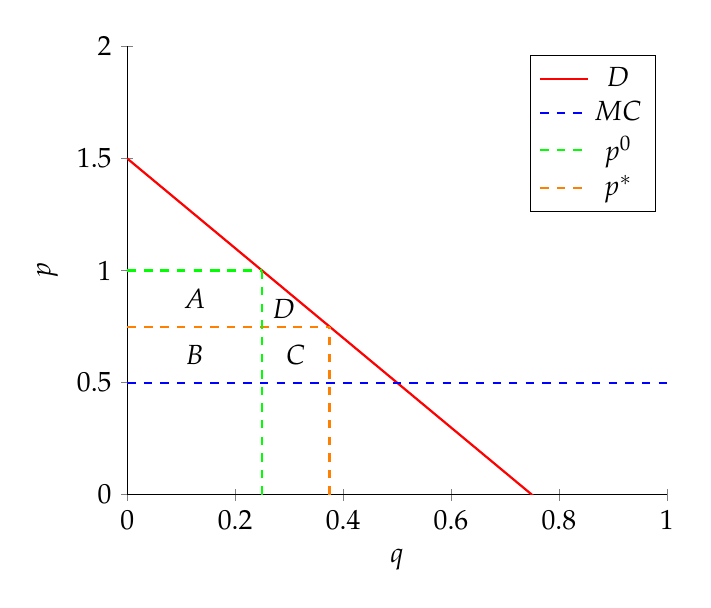
\begin{tikzpicture}[scale=1,thick]
    
          \begin{axis}[
              samples = 100,     		
              xmin = 0, xmax = 1,
              ymin = 0, ymax = 2,
              xlabel = $q$,
              ylabel = $p$,
              axis y line = left,    
              axis x line = bottom,
              y axis line style = {-}, 
              x axis line style = {-}
            ]
            
            \addplot[red,thick,
            domain=0:3,
            range = 0:3]{-2*x + 1.5};
            \addlegendentry{$D$};
            \addplot[blue,thick,dashed,
            domain=0:1,
            range = 0:3]{.5};
            \addlegendentry{$MC$};
            \addplot[green,thick,dashed,
            domain=0:.25,
            range = 0:3]{1};
            \addlegendentry{$p^0$};
            \addplot[orange,thick,dashed,
            domain=0:.375,
            range = 0:3]{.75};
            \addlegendentry{$p^*$};
            \draw [green,thick,dashed] (.25,0) -- (.25,1);
            \draw [orange,thick,dashed] (.375,0) -- (.375,.75);
            \node at (.125,.625) {$B$};
            \node at (.125,.875) {$A$};
            \node at (.3125,.625) {$C$};
            \node at (.29,.83) {$D$};
          \end{axis}
        \end{tikzpicture}
    \end{center}
    We first consider the firm's decision. If they move from $p^0$ to $p^*$, the increase in surplus is $C-A$, while they pay $z$. So in particular, they will change price when 
    \[C-A-z \geq 0\]
    However, the consumer surplus resulting from the price change is $A+D$. Then the total change in surplus from a change in price is given by
    \[(C-A) + (A+D) = C+D\]
    The issue arises when we have
    \[C+D \geq z \geq C-A\]
    The firm will not change price, but the increase in surplus exceeds the menu cost, so it's socially efficient for them to change price.
    \item Mankiw argues that this is likely to happen; the decision to change price has a first order effect on social surplus, and only a second order effect on the firm's profit. So the socially inefficient outcome is likely to happen because of the externality on consumer surplus. Consider, for example, a profit function $\pi(p)$ and a social welfare function $SW(p)$. If we Taylor expand $\pi(p_0)$ around $p^*$, we have
    \[\begin{split}
        \pi(p_0) &\approx \pi(p^*) + \underbrace{\pi'(p^*)(p_0 - p^*)}_{=0} + \frac{1}{2}\pi''(p^*)(p_0 - p^*)^2 \\
        &\approx \pi(p^*) + \frac{1}{2}\pi''(p^*)(p_0 - p^*)^2
    \end{split}\]
    However, if we do the same thing with the social welfare function, we have
    \[SW(p_0) \approx SW(p^*) + SW'(p^*)(p_0 - p^*) + \frac{1}{2}SW''(p^*)(p_0 - p^*)^2\]
    These conditions imply that
    \[\begin{split}
        \triangle \pi &= \pi(p_0) - \pi(p^*) \approx (p_0 - p^*)^2 \\
        \triangle SW &= SW(p_0) - SW(p^*) \approx (p_0 - p^*)
    \end{split}\]
    So given a menu cost $z$, a small shock $M^S$ is likely to result in an unchanged $P$, implying output adjustment and non-neutral money!
\end{itemize}

\subsection{Blanchard and Kiyotaki}

\begin{itemize}
    \item Use the Dixit-Stiglitz setup with differentiated goods. The firms exert aggregate demand externalities on one another.
    \item \textbf{Dixit-Stiglitz setup}: 
    \begin{itemize}
        \item Differentiated goods (CES utility, ideal variety and love for variety)
        \item Price setting power (monopolistic competition, $P > MC$)
        \item $N$ is large; each firm is small, so $\triangle P_i$ does not impact $\mathbb{P}$
        \item Free entry and exit, so long-run profit is 0. Note, however, that in the Blanchard-Kiyotaki model we assess, we focus on the short-run, so the number of firms is fixed at $\overline{N}$, so $\pi \neq 0$.
    \end{itemize}
    \item The monopolistic competition and differentiated goods give the price-setting decision to firms and justifies demand-determined output, implying that shocks to AD can impact output. At a given price, firms are willing to sell more because $P>MC$, quantity constrained by demand. Output is too low from a societal perspective. It implicitly also assumes that the labor market is not competitive -- the firms' output level determines the number of workers who are employed.
    \item There's an AD externality here. When a firm considers whether to lower its price, it will \textbf{increase} its own demand along its own demand curve. It will also \textbf{decrease} the overall price level and raise AD. 
    \begin{itemize}
        \item The impact of the increase in AD falls mostly on other firms, so an individual firm does not consider it when it makes its decision about whether or not to change price. 
        \item With a menu cost, it's possible that firms do not lower prices to the socially efficient level, so the overall price level and aggregate output is too low.
    \end{itemize}
    \item \textbf{Model setup}: 
    \begin{itemize}
        \item The continuum of household-producers on [0,1] face the problem
        \[\max\;U\left(\mathbb{C}_i, \frac{M_i}{\mathbb{P}}, L_i\right) = \left(\frac{\mathbb{C}_i}{\alpha}\right)^{\alpha}\left(\frac{M_i/\mathbb{P}_i}{1-\alpha}\right)^{1-\alpha} - \frac{L_i^{\beta}}{\beta}\]
        where
        \[\mathbb{C}_i = \left[\int_0^1C_{ij}^{\frac{\sigma - 1}{\sigma}}dj\right]^{\frac{\sigma}{\sigma-1}}\]
        Note that this is just the continuous analog to the discrete time version:
        \[\mathbb{C}_i = \left[C_1^{\frac{\sigma - 1}{\sigma}} + C_2^{\frac{\sigma - 1}{\sigma}} + \hdots + C_N^{\frac{\sigma - 1}{\sigma}}\right]^{\frac{\sigma}{\sigma-1}}\]
        This is a money-in-utility setup -- having cash makes you happy (seems kind of stupid but whatever).
        \item Production is given by
        \[Y_i = L_i\]
        \item An individual's budget constraint is given by
        \[P_iY_i = \int_0^1P_jC_{ij}dj + M_i\]
        \item Finally, the price index is given by
        \[\mathbb{P} = \left[\int_0^1P_j^{1-\sigma}dj\right]^{\frac{1}{1-\sigma}}\]
    \end{itemize}
    \item This is solved easily in three steps (stolen from Yu-Chin's file):
    \begin{enumerate}
        \item Denote consumption spending by $X_i$ and solve for the consumption demand for each good
        \item The household then picks between consuming and holding money
        \item Consider the household producer's production and pricing decisions, given the demand for their goods.
    \end{enumerate}
    \item \textbf{Step 1}: the household chooses consumption:
    \[\max_{C_{ij}}\; \left[\int_0^1C_{ij}^{\frac{\sigma - 1}{\sigma}}dj\right]^{\frac{\sigma}{\sigma-1}}\]
    subject to budget constraint
    \[X_i = \int_0^1P_jC_{ij}dj\]
    Noting that exponentiating functions is a monotonic transformation, we can remove the $\sigma / (\sigma - 1)$ exponent, so the Lagrange equation is given by
    \[\mathcal{L} = \int_0^1C_{ij}^{\frac{\sigma - 1}{\sigma}}dj + \lambda\left(X_i - \int_0^1P_jC_{ij}dj\right)\]
    This equation has infinite first order conditions, characterized by
    \[[C_{ij}] = \int_0^1\frac{\sigma - 1}{\sigma}C_{ij}^{-\frac{1}{\sigma}}dj - \lambda \int_0^1P_jdj = 0\]
    This condition implies that
    \[\frac{\sigma - 1}{\sigma}C_{ij}^{-\frac{1}{\sigma}} = \lambda P_j\quad \forall j\]
    So then the ratio of the first order conditions for two goods is
    \[\frac{C_{ij}}{C_{ik}} = \left(\frac{P_j}{P_k}\right)^{-\sigma}\]
    Then we note that we can exponentiate both sides by $(\sigma - 1) / \sigma$ and get
    \[\left(\frac{C_{ij}}{C_{ik}}\right)^{\frac{\sigma - 1}{\sigma}} = \left(\frac{P_j}{P_k}\right)^{1-\sigma}\]
    If we integrate by $j$ on both sides, we get:
    \begin{equation}\label{CES Consumption}
        \begin{split}
        &\int_0^1\left(\frac{C_{ij}}{C_{ik}}\right)^{\frac{\sigma - 1}{\sigma}}dj = \int_0^1\left(\frac{P_j}{P_k}\right)^{1-\sigma}dj \\
        \implies &\frac{1}{C_{ik}^{\frac{\sigma - 1}{\sigma}}}\int_0^1C_{ij}^{\frac{\sigma - 1}{\sigma}}dj = \frac{1}{P_k^{1-\sigma}}\int_0^1P_j^{1-\sigma}dj \\
        \implies &\frac{\mathbb{C}_i^{\frac{\sigma - 1}{\sigma}}}{C_{ik}^{\frac{\sigma - 1}{\sigma}}} = \frac{\mathbb{P}^{1-\sigma}}{P_k^{1-\sigma}} \\
        \implies &\left(\frac{\mathbb{C}_i}{C_{ik}}\right)^{-\sigma} = \frac{\mathbb{P}}{P_k}
    \end{split}
    \end{equation}
    This condition dictates the allocation of consumption spending to different goods. So the household solves a two-step problem: first, figure out how much of your budget goes to holding money, and how much to consumption. Once the consumption fraction has been allocated ($\mathbb{C}_i$ determined), the allocation is given by the relative price of goods.
    \item \textbf{Step 2}: decide the relative allocation of $\mathbb{C}_i$ and $M_i$. The problem is then
    \[\mathcal{L} = \left(\frac{\mathbb{C}_i}{\alpha}\right)^{\alpha}\left(\frac{M_i/\mathbb{P}}{1-\alpha}\right)^{1-\alpha} - \frac{L_i^{\beta}}{\beta} + \lambda(P_iY_i + \overline{M}_i -\mathbb{C}_i\mathbb{P} - M_i)\]
    This has first order conditions
    \[\begin{split}
        [\mathbb{C}_i]:\;& \left(\frac{\mathbb{C}_i}{\alpha}\right)^{\alpha-1}\left(\frac{M_i/\mathbb{P}}{1-\alpha}\right)^{1-\alpha} - \lambda \mathbb{P} = 0 \\
        [M_i]:\;& \frac{1}{\mathbb{P}}\left(\frac{\mathbb{C}_i}{\alpha}\right)^{\alpha}\left(\frac{M_i/\mathbb{P}}{1-\alpha}\right)^{-\alpha}-\lambda = 0
    \end{split}\]
    Combining these expressions implies that
    \[\frac{\mathbb{C}_i}{\alpha} = \frac{M_i/\mathbb{P}}{1-\alpha}\]
    Substituting back into the budget constraint yields
    \[\begin{split}
        &P_iY_i + \overline{M}_i = \mathbb{C}_i\mathbb{P}_i + M_i \\
        \implies &P_iY_i + \overline{M}_i = \mathbb{C}_i\mathbb{P}_i + \frac{1-\alpha}{\alpha}\mathbb{P}\mathbb{C}_i \\
        \implies &P_iY_i + \overline{M}_i = \frac{\mathbb{P}\mathbb{C}_i}{\alpha} \\
        \implies &\mathbb{P}\mathbb{C}_i = \alpha\left(P_iY_i + \overline{M}_i\right)
    \end{split}\]
    And putting this condition back into the budget constraint:
    \[\begin{split}
        &P_iY_i + \overline{M}_i = \mathbb{C}_i\mathbb{P}_i + M_i \\
        \implies &P_iY_i + \overline{M}_i = \alpha\left(P_iY_i + \overline{M}_i\right) + M_i \\ 
        \implies &M_i = (1-\alpha)\left(P_iY_i + \overline{M}_i\right)
    \end{split}\]
    Finally, the ratio of these conditions yields
    \[\frac{\mathbb{P}\mathbb{C}_i}{M_i} = \frac{\alpha}{1-\alpha}\]
    Then using equation (\ref{CES Consumption}), we can write
    \[\frac{\mathbb{P}}{M_i}\left(\frac{\mathbb{P}}{P_k}\right)^{-\frac{1}{\sigma}}C_{ik} = \frac{\alpha}{1-\alpha}\implies \boxed{C_{ik} = \frac{\alpha}{1-\alpha}\frac{M_i}{\mathbb{P}}\left(\frac{P_k}{\mathbb{P}}\right)^{-\frac{1}{\sigma}}}\]
    This condition relates the consumption of an individual good to the agent's consumption of real money and the relative price of the good. The real money acts as a scalar to consumption of all types $k$, while the relative price denotes the relative weight of the individual good.
    \item \textbf{Step 3}: make the decision about labor. Using the conditions found above for consumption and money holdings, rewrite the utility function:
    \[\begin{split}
        U &= \left(\frac{\mathbb{C}_i}{\alpha}\right)^{\alpha}\left(\frac{M_i/\mathbb{P}}{1-\alpha}\right)^{1-\alpha} - \frac{L_i^{\beta}}{\beta} \\
        &= \left(\frac{P_iY_i + \overline{M}_i}{\mathbb{P}}\right)^{\alpha}\left(\frac{P_iY_i + \overline{M}_i}{\mathbb{P}}\right)^{1-\alpha} - \frac{L_i^{\beta}}{\beta} \\
        &= \frac{P_i}{\mathbb{P}}Y_i - \frac{Y_i^{\beta}}{\beta} + \frac{\overline{M}_i}{\mathbb{P}}
    \end{split}\]
    In general equilibrium, production must equal consumption, so we have
    \[\begin{split}
        Y_i &= \int_0^1C_{ik}dk \\
        &= \int_0^1\frac{\alpha}{1-\alpha}\frac{M_i}{\mathbb{P}}\left(\frac{P_k}{\mathbb{P}}\right)^{-\frac{1}{\sigma}}dk \\
        &= \frac{\alpha}{1-\alpha}\frac{M}{\mathbb{P}}\left(\frac{P_i}{\mathbb{P}}\right)^{-\frac{1}{\sigma}}
    \end{split}\]
    We note that price and quantity are inversely related, so we have a downward-sloping demand curve. In particular, note that if we write
    \begin{equation}\label{CES Demand}
        Y_i = D\left(\frac{M}{\mathbb{P}},\frac{P_i}{\mathbb{P}}\right)
    \end{equation}
    we have that output is increasing in real money and decreasing in real prices.
    \item Consider a negative monetary shock. By the above, demand shifts to the left. We visualize this graph below:
    \begin{center}
        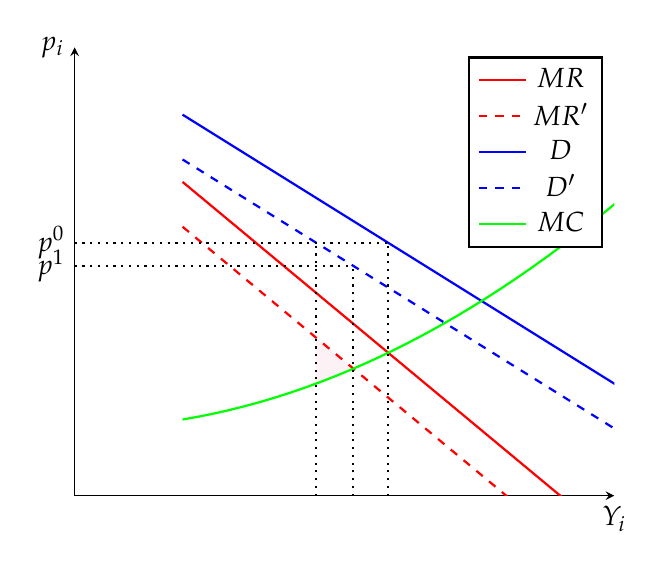
\begin{tikzpicture}[scale=1,thick]
    
          \begin{axis}[
              samples = 100,     		
              xmin = 0, xmax = 1,
              ymin = 0, ymax = 2,
              xlabel = $Y_i$,
              ylabel = $p_i$,
              xticklabels={,,},
              yticklabels={,,},
              x tick label style={major tick length=0pt},
              y tick label style={major tick length=0pt},
              axis y line = left,    
              axis x line = bottom,
              every axis x label/.style={
                    at={(ticklabel* cs:1)},
                    anchor=north,
                },
                every axis y label/.style={
                    at={(ticklabel* cs:1)},
                    anchor=east,
                },
              extra y ticks={1.026, 1.129},
              extra y tick labels={$p^1$, $p^0$}
            ]
            
            \addplot[red,thick,
            domain=.2:3,
            range = 0:3]{-2*x + 1.8};
            \addlegendentry{$MR$};
            \addplot[name path=mr,red,thick,dashed,
            domain=.2:3,
            range = 0:3]{-2*x + 1.6};
            \addlegendentry{$MR'$};
            \addplot[blue,thick,
            domain=.2:3,
            range = 0:3]{-1.5*x + 2};
            \addlegendentry{$D$};
            \addplot[blue,thick,dashed,
            domain=.2:3,
            range = 0:3]{-1.5*x + 1.8};
            \addlegendentry{$D'$};
            \addplot[name path=mc,green,thick,
            domain=.2:3,
            range = 0:3]{x^2 + .3};
            \addlegendentry{$MC$};
            \addplot[
                thick,
                color=purple,
                fill=purple, 
                fill opacity=0.05
            ]
            fill between[
                of=mr and mc,
                soft clip={domain=.447:.516},
            ];
            \draw [black,thick,dotted] (.516,0) -- (.516,1.026);
            \draw [black,thick,dotted] (0,1.026) -- (.516,1.026);
            \draw [black,thick,dotted] (.581,0) -- (.581,1.129);
            \draw [black,thick,dotted] (0,1.129) -- (.581,1.129);
            \draw [black,thick,dotted] (.447,0) -- (.447,1.129);
          \end{axis}
        \end{tikzpicture}
    \end{center}
    Should the firm transition from $p^0$ to $p^1$? We first consider the case with no menu costs. In this case, it is costless for the firms to transition (all are identical), which means that they will change price. The lower aggregate price level will increase real money, which in turn will increase output (see equation (\ref{CES Demand})), which will return push the demand curve back to its original location, and the economy will return to its previous equilibrium. However, if there are menu costs $z$, then the shaded area comes into play. If that shaded area is larger than the menu cost, then the firms will change price (the surplus benefit is larger to them than the menu cost). However, if this menu cost is larger than that area, they will not change price. In this case, output drops and real money balances drop.
    \item Generally speaking, if there is a menu cost, a firm considering a price change recognizes that it will increase its own demand as well as increase aggregate demand. However, they do not care about the second shift (externality), so with a menu cost, firms may not lower prices to the socially efficient amount, which results in artificially high $\mathbb{P}$ and artificially low aggregate output.
    \item This gives the monetary non-neutrality result. See the demand curve given by equation (\ref{CES Demand}). If there is a monetary shock, with no corresponding price change, output will change, so money impacts output.
    \item Further, there is a \textbf{pro-cyclical} real wage: 
    \[Y\downarrow \implies L \downarrow \implies \frac{w}{\overline{P}} \downarrow\]
    \item There is then a justification for a small monetary expansion, as this can raise output towards the socially optimal level (needs to surpass the menu cost).
    \item Large shocks have social cost, as firms have to pay the menu cost to change price.
    \item \textbf{Ball and Romer critique}: we know that empirically, labor supply is inelastic. This means that a small change in labor supply leads to a large change in real wage. Graphically, this means that aggregate supply is fairly steep. Consider a small monetary contraction:
    \[M\downarrow \implies \overline{P}_i \implies \overline{\mathbb{P}} \implies \frac{M}{\mathbb{P}} \downarrow \implies Y \downarrow \implies L^D \downarrow \iff L^S \downarrow\]
    If labor demand shifts left, then in the competitive labor market, wage must decrease. Correspondingly,
    \[w \downarrow \implies MC \downarrow\]
    However, a decrease in MC means that the size of the triangle is larger than we thought earlier!
    \begin{center}
        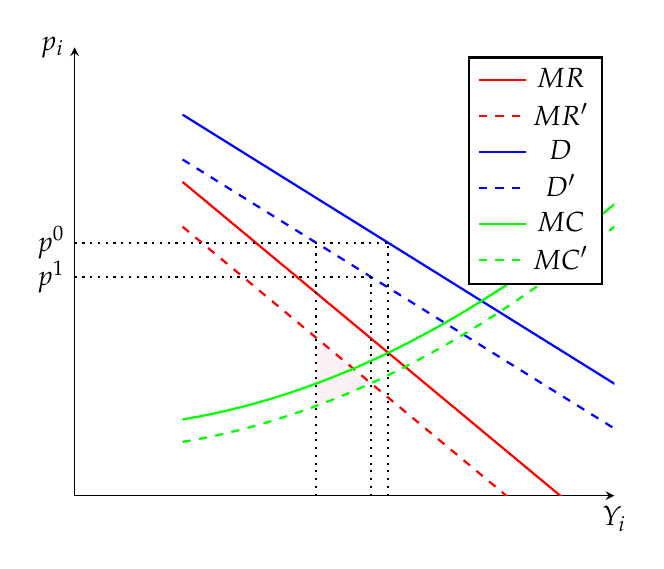
\begin{tikzpicture}[scale=1,thick]
    
          \begin{axis}[
              samples = 100,     		
              xmin = 0, xmax = 1,
              ymin = 0, ymax = 2,
              xlabel = $Y_i$,
              ylabel = $p_i$,
              xticklabels={,,},
              yticklabels={,,},
              x tick label style={major tick length=0pt},
              y tick label style={major tick length=0pt},
              axis y line = left,    
              axis x line = bottom,
              every axis x label/.style={
                    at={(ticklabel* cs:1)},
                    anchor=north,
                },
                every axis y label/.style={
                    at={(ticklabel* cs:1)},
                    anchor=east,
                },
              extra y ticks={.977, 1.129},
              extra y tick labels={$p^1$, $p^0$}
            ]
            
            \addplot[red,thick,
            domain=.2:3,
            range = 0:3]{-2*x + 1.8};
            \addlegendentry{$MR$};
            \addplot[name path=mr,red,thick,dashed,
            domain=.2:3,
            range = 0:3]{-2*x + 1.6};
            \addlegendentry{$MR'$};
            \addplot[blue,thick,
            domain=.2:3,
            range = 0:3]{-1.5*x + 2};
            \addlegendentry{$D$};
            \addplot[blue,thick,dashed,
            domain=.2:3,
            range = 0:3]{-1.5*x + 1.8};
            \addlegendentry{$D'$};
            \addplot[green,thick,
            domain=.2:3,
            range = 0:3]{x^2 + .3};
            \addlegendentry{$MC$};
            \addplot[name path=mc,green,thick, dashed,
            domain=.2:3,
            range = 0:3]{x^2 + .2};
            \addlegendentry{$MC'$};
            \addplot[
                thick,
                color=purple,
                fill=purple, 
                fill opacity=0.05
            ]
            fill between[
                of=mr and mc,
                soft clip={domain=.447:.549},
            ];
            \draw [black,thick,dotted] (.549,0) -- (.549,.977);
            \draw [black,thick,dotted] (0,.977) -- (.549,.977);
            \draw [black,thick,dotted] (.581,0) -- (.581,1.129);
            \draw [black,thick,dotted] (0,1.129) -- (.581,1.129);
            \draw [black,thick,dotted] (.447,0) -- (.447,1.129);
          \end{axis}
        \end{tikzpicture}
    \end{center}
    Basically, given the inelastic nature of labor supply, this shift in MC should be big, which means that the surplus gains from changing price should also be very large. This means that the story that firms won't change prices is implausible unless menu costs are very large, which is also implausible.
    \item \textbf{Fixes}: maybe there are short-run labor market imperfections. In the short-run, real wages are sticky, and the labor market does not adjust with labor supply. In that case, in the example from before, when labor demand drops, L drops as well, but wage doesn't respond dramatically. 
    \item How do we model disequilibrium real wage? We use \textbf{real rigidities}:
    \begin{itemize}
        \item TODO (lecture?)
        \item Shapiro-Stiglitz: imperfect monitoring. The result is that the short run real wage is rigid, and the labor market off of the inelastic long run labor supply curve means that the labor market does not clear.
    \end{itemize}
\end{itemize}

\subsection{Shapiro-Stiglitz Efficiency Wage Model}

\begin{itemize}
    \item \textbf{Model setup}
    \begin{itemize}
        \item Continuous time, and all agents are risk-neutral and infinitely lived. Workers care about wages $w$ and effort $e$. There are only two effort levels: exerting effort ($e_t = \overline{e}$) or shirking ($e_t = 0$). 
        \item There is imperfect information. If effort were observable, the firm would write contracts that are effort-contingent. However, observing effort is impossible, and as a result, the firms can only observe the aggregate output. 
        \item This is a moral hazard problem -- effort cannot be observed and there is limited liability (no punishment for individual low output), so workers must be incentivized to exert effort.
        \item The utility of the worker is given by
        \[u(t) = \begin{cases}
        w(t) - e(t) & \text{if employed} \\
        0 & \text{if unemployed}
        \end{cases}\]
        Here, $w(t)$ is a real wage. Then workers attempt to maximize lifetime utility given by
        \[\max_{e(t) \in \{0, \overline{e}\}}\; \int_{t=0}^{\infty} e^{-\rho t}u(w(t), e(t))dt\]
        \item At each value of $t$, workers are in one of three possible states:
        \begin{enumerate}
            \item NS (Employed and Not Shirking, $e = \overline{e}$): $V_E^{NS}$
            \item S (Employed and Shirking, $e = 0$): $V_E^S$ 
            \item U (Unemployed): $V_U$
        \end{enumerate}
        Further, there are probabilities (technically flow rates) of transitioning between the states. In particular, if employed, there is probability $b$ of being fired regardless of effort, if shirking, an additional probability $q$ of being caught and fired. Further, there is an endogenous (to economy, not individual) probability $a$ of finding a job at each time $t$. So then the transition probabilities are:
        \[\begin{split}
            P(NS \rightarrow U)&: b \\
            P(S \rightarrow U)&: b+q \\
            P(U \rightarrow \{NS, S\})&: a
        \end{split}\]
        The firm faces the problem
        \[\max_{L(t)}\; F(\overline{e}L(t)) - w(t)[L(t) + S(t)]\]
        where $L(t)$ is the number of non-shirking workers, and $S(t)$ is the number of shirkers. Finally, there are $N$ total firms and the population of workers is $\overline{L}$.
    \end{itemize}
    \item If a worker is employed and not shirking, then their payoff/value function (sort of like an HJB I think) is given by
    \[\begin{split}
        V^{NS} &= \underbrace{(w-\overline{e})dt}_{\text{flow payoff}} + \underbrace{(1-\rho dt)}_{\text{discounting}}\underbrace{\left[(1-bdt)V^{NS} + bdtV^{U}\right]}_{\text{continuation payoff}} \\
        \implies V^{NS} &= \frac{(w-\overline{e})dt + (1-\rho dt)bdt\cdot V^U}{1-(1-\rho dt)(1-b dt)}
    \end{split}\]
    We then take the limit as $dt \to 0$ using L'Hôpital's rule:
    \begin{equation}\label{NS HJB}
        \begin{split}
            \lim_{dt \to 0}V^{NS} &= \lim_{dt \to 0}\frac{(w-\overline{e})dt + (1-\rho dt)bdt\cdot V^U}{1-(1-\rho dt)(1-b dt)} \\
            &= \lim_{dt \to 0} \frac{w-\overline{e} +(b-2b\rho dt)V^U}{\rho + b -2\rho b dt} \\
            &= \frac{w-\overline{e} +bV^U}{\rho + b} \\
            \implies \rho V^{NS} &= w-\overline{e} + b(V^U-V^{NS})
        \end{split}
    \end{equation}
    We note that if we use this equation (\ref{NS HJB}) as a reference, the only difference between $V^{NS}$ and $V^S$ is the flow payoff $\overline{e} \to 0$ and the rate of being fired $b \to b+q$. So following a similar derivation, we have
    \begin{equation}\label{S HJB}
        \rho V^{S} = w + (b+q)(V^U-V^S)
    \end{equation}
    To get the unemployed value function, we use a similar idea/approach (not derived here) to get to
    \begin{equation}\label{U HJB}
        \rho V^U = a(V^E - V^U)
    \end{equation}
    where $V^E \in \{V^{NS}, V^S\}$.
    \item From the firm's optimization, we know that as long as $F(\overline{e}L(t)) \geq w(t)$, the firm will want to pay a wage where there is no incentive to shirk, i.e. a wage $w^*$ such that
    \[V^{NS} = V^S = V^E\]
    \item We assess the steady state of this model. In particular, this means that there is no net change in labor force participation. Correspondingly, as jobs are created at the same rate as jobs are destroyed, it must be the case that
    \begin{equation}\label{Shapiro Labor SS}
        \underbrace{a(\overline{L} - NL)}_{\text{hired unemployed}} = \underbrace{bNL}_{\text{fired workers}}
    \end{equation}
    \item Using equations (\ref{NS HJB}) and (\ref{S HJB}), we have that
    \[\begin{split}
        &V^NS = V^S \\
        \implies &w-\overline{e} + b(V^U-V^E) = w + (b+q)(V^U-V^E) \\
        \implies &\overline{e} = q(V^E - V^U) \\
        \implies &V^E - V^U = \frac{\overline{e}}{q} > 0
    \end{split}\]
    This is the \textbf{employment premium}; workers prefer being employed to being unemployed. Substituting the employment premium into (\ref{U HJB}) yields $V^U$:
    \[\begin{split}
        V^U &= \frac{a}{\rho}(V^E - V^U) \\
        &= \frac{a}{\rho}\frac{\overline{e}}{q}
    \end{split}\]
    Substituting into the employment premium condition:
    \[\begin{split}
        V^E &= \frac{\overline{e}}{q} + V^U \\
        &= \frac{\overline{e}}{q}\left(1 + \frac{a}{\rho}\right) \\
        &= \frac{\overline{e}}{q}\left(\frac{a + \rho}{\rho}\right) \\
    \end{split}\]
    Now taking equation (\ref{NS HJB}):
    \[\begin{split}
        &V^E = \frac{w^* - \overline{e} + bV^U}{\rho + b} \\
        \implies &w^* = (\rho + b)V^E - bV^U + \overline{e} \\
        \implies &w^* = \rho V^E + b\left(\frac{\overline{e}}{q}\right) + \overline{e} \\
        \implies &w^* = \rho \left(\frac{\overline{e}}{q}\left(\frac{a + \rho}{\rho}\right)\right) + b\left(\frac{\overline{e}}{q}\right) + \overline{e} \\
        \implies &w^* = \left(a + b+ \rho\right)\left(\frac{\overline{e}}{q}\right) + \overline{e} \\
    \end{split}\]
    Now, we note that using equation (\ref{Shapiro Labor SS}), we have
    \[\begin{split}
        a + b &= b\left(\frac{NL}{\overline{L}-NL} +1\right) \\
        &= \frac{b\overline{L}}{\overline{L} - NL}
    \end{split}\]
    So combining this condition with the wage condition, we have the \textbf{No-Shirking Condition}, or the minimum wage required to induce $\overline{e}$:
    \begin{equation}\label{No-Shirking Condition}
        w^* = \overline{e} + \left(\rho + \frac{b\overline{L}}{\overline{L} - NL}\right)\frac{\overline{e}}{q}
    \end{equation}
    \item Now consider what the labor market looks like. In particular, note that in a competitive labor market and in the absence of the information asymmetry, firms will offer the first-best contract, where $w = \overline{e}$. Workers are indifferent between working and not working, and any wage above this will result in full labor force participation. However, firms offer a wage off of this schedule; firms will offer $w^*$, i.e. the wage to incentivize everyone to not shirk. So the market looks like this:
    \begin{center}
        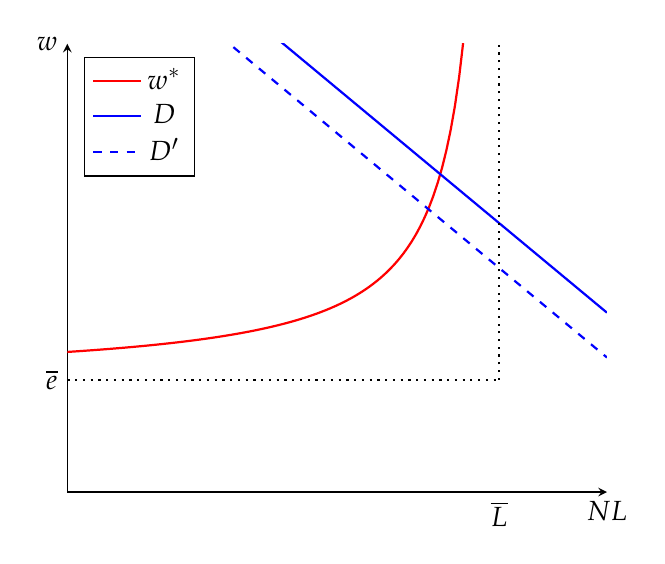
\begin{tikzpicture}[scale=1,thick]
    
          \begin{axis}[
              samples = 100,     		
              xmin = 0, xmax = 1,
              ymin = 0, ymax = 2,
              xlabel = $NL$,
              ylabel = $w$,
              xticklabels={,,},
              yticklabels={,,},
              x tick label style={major tick length=0pt},
              y tick label style={major tick length=0pt},
              axis y line = left,    
              axis x line = bottom,
              every axis x label/.style={
                    at={(ticklabel* cs:1)},
                    anchor=north,
                },
                every axis y label/.style={
                    at={(ticklabel* cs:1)},
                    anchor=east,
                },
              extra y ticks={.5},
              extra y tick labels={$\overline{e}$},
              extra x ticks={.8},
              extra x tick labels={$\overline{L}$},
              legend pos = north west
            ]
            \addplot[red,thick,
            domain=0:.79,
            range = 0:3]{.5 + (1/(.8-x))*.1};
            \addlegendentry{$w^*$}
            \addplot[blue,thick,
            domain=0:1,
            range = 0:3]{-2*x + 2.8};
            \addlegendentry{$D$}
            \addplot[blue,thick,dashed,
            domain=0:1,
            range = 0:3]{-2*x + 2.6};
            \addlegendentry{$D'$}
            \draw [black,thick,dotted] (0, .5) -- (.8, .5);
            \draw [black,thick,dotted] (.8,.5) -- (.8,2);
          \end{axis}
        \end{tikzpicture}
    \end{center}
    Note that for the shift from $D$ to $D'$, the change in $w$ is less on the $w^*$ curve than on the competitive equilibrium curve. This yields the result that we're interested in: a shift in labor demand yields a smaller-than-competitive shift in wage. This model is \textbf{micro-founded} in imperfect information.
    \item We can also use the No-Shirking Condition, equation (\ref{No-Shirking Condition}), to do comparative statics with the model. For example, 
    \[NL \to \overline{L} \implies w^* \to \infty\]
    so as we approach full employment, wage explodes. If we add the production function $Y = Af(L)$, then we have that in the equilibrium,
    \[w = Af'(L)\]
    So 
    \[A \uparrow \implies UE \downarrow \implies w^* \uparrow\]
    \item \textbf{Empirical Evidence}: there are substantial inter-industry wage differentials due to differences in $q$. Krueger showed that there were higher wages and steeper tenure premia in company-owned fast food restaurants than franchised ones. Cappelli and Chauvin also show that within the same auto manufacturer, higher wage premium plants have fewer discipline dismissals. 
\end{itemize}

\subsection{McCall Search Model}

\begin{itemize}
    \item How do we model unemployment? If unemployment is a leisure choice, this isn't interesting -- we need labor market frictions to force us to have involuntary unemployment. Then we can ask whether the current level of employment is efficient or not, as well as assess the distribution of wages. To do this, we'll use dynamic programming. 
    \item \textbf{Model setup}: We have risk-neutral individuals who are presented with some wage $w \in W$ where $W$ has bounded support $f(w)$. Further, $w_t$ is i.i.d. for individuals. The choice that the agent makes each period is to accept the wage offer (and make it for the rest of time) or reject the wage offer and receive another offer the following period. Finally, there's discounting, such that the problem faced by the agent is
    \[\max_{\text{Accept, Reject}}\;\sum_{t=0}^{\infty} \beta^tc_t\]
    Here, the consumption is either the wage (if a wage has been accepted) or some unemployment benefit $b$. This is an example of \textbf{undirected search} (can't try to find wages in particular parts of the distribution). The search is \textbf{without recall} (can't get the wage offer back if rejected) and without firing (make the wage forever).
    \item We can solve a simpler version of this problem. Every period you receive a wage offer $X \in [0,1]$. Your discount rate is $\beta = e^{-\rho} = .9$, and you're risk neutral. You get a one-period payoff.
    \item This can be formulated as a dynamic programming problem. Define the value function as 
    \[v(x_0) = \max_{\text{Accept, Reject}}\; \left\{x_0, \beta E[V(x_1)]\right\}\]
    We want to find a policy, which will be a threshold function (which can apparently be shown formally). This just means that we're looking for 
    \[g(x) = \begin{cases}
    \text{Accept} & x \geq x^* \\
    \text{Reject} & x < x^*
    \end{cases}\]
    Correspondingly, we can write the value function as 
    \[v(x) = \begin{cases}
    x & x \geq x^* \\
    \beta E[v] = \underline{v} & x < x^*
    \end{cases}\]
    \item Noting that we have indifference at the threshold (more on this in spring quarter), we have that at the threshold offer $x^*$, we have that 
    \[\begin{split}
        w^* &= \beta E[v] \\
        &= \beta\left(\int_0^{w^*}w^*f(x)dx + \int_{w^*}^1xf(x)dx\right) \\
        &= \beta \left(w^{*2} + \frac{1 - w^{*2}}{2}\right) \\
        &= \beta \left(\frac{1 + w^{*2}}{2}\right)
    \end{split}\]
    Then you can solve the quadratic and get
    \[w^* = \frac{1 - \sqrt{1-\beta^2}}{\beta}\]
    To change to McCall, we have to add a general PDF $f(w)$ and a payoff for the rest of time insted of only one period. In this case, we have that
    \[v(w_t) = \max_{\text{Accept, Reject}}\; \left\{\frac{w_t}{1-\beta}, b + \beta E[V(w_{t+1})]\right\}\]
    So we can write that, at the threshold, the value of accepting is equal to the value of waiting, which means that
    \[V^A = b + \beta E[V]\]
    The value of accepting is the infinite sum of future discounted wages, and the expectation of future value is 
    \[E[V] = P(V^A) \times V^A + P(V^R) \times V^R\]
    The acceptance term is straightforward -- it's just the conditional expectation of $\frac{w}{1-\beta}$, given that $w \geq R$. The value of rejection is just receiving the reservation wage for the rest of time, given by $\frac{R}{1-\beta}$. So we can write
    \[\begin{split}
        \frac{R}{1-\beta} &= \underbrace{\int_{w<R}\frac{R}{1-\beta}dF(w)}_{\text{Reject}} + \underbrace{\int_{w\geq R}\frac{R}{1-\beta}dF(w)}_{\text{Accept}} \\
        &= b + \beta\left[\int_{w < R}\frac{R}{1-\beta}dF(w) + \int_{w\geq R} \frac{w}{1-\beta}dF(W)\right]
    \end{split}\]
    This implies that
    \begin{equation}\label{McCall Equilibrium}
        \underbrace{R-b}_{\text{Cost of Rejecting $R$}} = \frac{\beta}{1-\beta}\underbrace{\left[\int_{w\geq R}(w-R)dF(w)\right]}_{\text{expected benefit of next search}}
    \end{equation}
    How does this condition change for a mean-preserving spread? $R$ increases (TODO). To see this, note that
    \begin{equation}\label{Mean Preserving Spread}
        \begin{split}
        &R-b = \frac{\beta}{1-\beta}\left[\int_{w\geq R}(w-R)dF(w)\right] \\
        \implies &(1-\beta)(R-b) = \beta \left[\int_{w\geq R}(w-R)dF(w)\right] \\
        \implies &(1-\beta)(R-b) +\beta\left[\int_0^R(w-R)dF(w)\right] = \beta\left[ \int_0^{\overline{W}}wf(w)dw - R\right] \\
        \implies &R - (1-\beta)b +\beta\left[\int_0^R(w-R)dF(w)\right] = \beta E[w] \\
        \implies &R - b +\beta\left[\int_0^R(w-R)dF(w)\right] = \beta \left(E[w] - b\right)
    \end{split}
    \end{equation}
    \item As we said earlier, we want to incorporate unemployment into the model. Consider a continuum 1 of identical individuals sampling jobs from the same stationary distribution $F(w)$ of wages. When a job is created, it lasts until the worker dies, which happens with probability $s$, which is invariant across individuals. A proportion of population $s$ workers are born each period, so the population does not change, and new workers begin as unemployed. Because of the possibility of death, the effective discount factor of workers is $\beta(1+s)$. Correspondingly, the value of having accepted a wage of $w_t$ is given by
    \[V^A = \frac{w_t}{1 - \beta(1-s)}\]
    If the problem is set up and solved with this new discount factor, we just need to substitute it into equation (\ref{McCall Equilibrium}) to get
    \[R - b = \frac{\beta(1-s)}{1 - \beta(1-s)}\left[\int_{w\geq R}(w-R)dF(w)\right]\]
    So this doesn't really change the problem in an interesting way, it just changes the discount factor.
    \item The Flow Approach to Unemployment: take $U_t$ to be the number of unemployed workers at time $t$. Each $t$, $s$ new workers are born into the unemployment pool, and out of the $U_t$ unemployed workers, those who survive and don't find a job remain unemployed. Then $U_t$ evolves by
    \[U_{t+1} = \underbrace{s}_{\text{new workers}} + \underbrace{(1-s)}_{\text{survive}}\underbrace{F(R)}_{\text{reject offer}}U_t\]
    At steady state, the unemployment level does not change, which means that 
    \[U_t = U_{t+1} \implies \overline{U} = \frac{s}{1-(1-s)F(R)} = \frac{\overbrace{s}^{\text{job destruction rate}}}{\underbrace{s}_{\text{new workers}} + \underbrace{(1-s)(1-F(R))}_{\text{alive, accept job offer}}}\]
    We can perform comparative statics on this equation; in particular, we can see that $s \uparrow \implies \overline{U} \uparrow$ and $R \uparrow \implies \overline{U} \uparrow$.
    \item \textbf{Critiques}: 
    \begin{enumerate}
        \item The really important one is the \textbf{Rothschild Critique}. Essentially, Rothschild points out that the wage distribution will be degenerate if firms are profit-maximizing. The logic is that the setup assumes that firms face costly job posting and that every wage in the support $\overline{W}$ is offered. However, Rothschild points out that it's irrational to have profit-maximizing firms offering all the wages in this support. In particular, firms know that workers will accept any wage higher than the reservation wage $R$; if they offer a wage less than $R$, they waste the job-posting cost. If they offer any wage higher than $R$, they lose out on surplus. These two facts imply that $F(w)$ will have a unit mass at $R$. So there's no distribution and no search -- every firm offers $R$, and every worker will accept $R$ when offered.
        \item The \textbf{Diamond Paradox} also points out that in the economy described by Rothschild's Critique, for all $\beta < 1$, the unique equilibrium in the economy is $R = b$, and all workers accept their first wage offer. We simplify the above by setting $b=0$ without loss of generality. In this game, if every firm offers $R$, then the question is whether an individual firm has profitable deviation. If they offer $R-\varepsilon$, the problem facing the agent is then 
        \[V^A = \frac{R - \varepsilon}{1-\beta} \quad \text{vs.} \quad \beta \frac{R}{1-\beta} = V^R\]
        As
        \[\lim_{\varepsilon \to 0}V^A = \frac{R}{1-\beta} > \frac{\beta R}{1-\beta}\]
        we know that there must exist some $\varepsilon$ sufficiently small such that the worker prefers to accept the offer that's below the reservation wage. Firms can continue to deviate down to the unemployment benefit $b$ (0 in this case), which yields the Diamond result. Another way to see this is that in the economy characterized by the degenerate wage distribution, equation (\ref{McCall Equilibrium}) implies that
        \[R-b = \frac{\beta}{1-\beta}(1-F(R))(w - R)\]
        First, note that if $w = R$, then $R = b$, which is the Diamond result. However, note further that in this condition, rearranging in terms of $w$ yields
        \[w = R + \frac{(1-\beta)(R-b)}{\beta(1-F(R))}\]
        Then, 
        \[\frac{\partial w}{\partial R} = 1+\frac{\beta(1-F(R))(1-\beta) + (1-\beta)(R-b)\beta f(R)}{\left(\beta(1-F(R))\right)^2} > 0\]
        So if $w$ decreases in this economy, $R$ will also decrease, up until $R$ is driven to $b$. Any wage above $b$ cannot be an equilibrium. Further, according to \href{https://faculty.georgetown.edu/albrecht/SJE\%20Survey.pdf}{James Albrecht's paper on the 2010 Nobel Prize in Search Theory}:
        \begin{quote}
            The situation is even ``worse" if there is a monetary cost of search. In that case, unless the first search step is free -- an assumption that is made in many equilibrium search models -- no equilibrium exists.
        \end{quote}
    \end{enumerate}
    \item \textbf{Solutions to the Diamond Paradox}: If we assume that $F(w)$ is not the distribution of wages, but the distribution of ``fruits" exogeneously offered by ``trees", we resolve the paradox, but can't do anything interesting (no policy questions answered). If we introduce other dimensions of heterogeneity, like firm productivity, we can resolve the paradox; firms will have differential willingness to pay workers, so we get a distribution. If there's directed search, signaling can occur and workers can target different parts of the wage distribution according to productivity. Finally, and most importantly, we can modify the wage determination assumption, and assume that workers bargain, as opposed to just being forced to accept or reject the wage posting. This is the foundation of the Diamond-Mortensen-Pissarides model for which the Nobel Prize was awarded in 2010. In this model, wages are determined by Nash bargaining. The major shortcoming of this approach is that there's a reduced form matching function. I believe this is essentially the job search model covered in 509, but need to confirm (TODO). 
\end{itemize}

\subsection{Caplin-Spulber Model of Price Adjustment}

\begin{itemize}
    \item When we consider the dynamic adjustment process when assuming nominal rigidity, we need to reconcile microeconomic evidence of price changing frequency (pretty infrequent) with the high persistence of the effect of monetary policy in macroeconomic data. One way to approach this is to do state-contingent price adjustment: this is the Caplin-Spulber approach. They attempt to answer the question ``if price adjustments are endogeneous, what is the real effect of money?" They show that the existence of menu costs is insufficient for aggregate nominal price stickiness, although the results are not robust. The technique that they use is known as s-S, which is used in investment and inventory literature. 
    \item \textbf{Model Setup}: there are heterogeneous firms who face a menu cost. The initial distribution of prices is uniform on the interval $[M-s, M+s]$, so the aggregate price is $P = M$. Additionally, $p_i^* = M$, but because of menu costs, a given firm may not price at exactly $p_i = M$; rather, they will not change price so long as $p_i \in [M-s, M+s]$. 
    \item Given some small shock $M \rightarrow M'$, only some firms will change price; in particular, those whose prices no longer fall in the interval $[M'-s, M'+s]$. However, because of the menu costs, firms who adjust may not adjust to $M'$; rather, they adjust according to the expected future path of $M$ (you want to within the interval as much as possible to avoid paying menu cost to change price). So in this model, if firms expect $M$ to continue to increase, they will select large and infrequent price adjustments. For example, if firms are positive that $M$ will monotonically increase in time, optimal price setting policy (given sufficiently large menu cost) is to price at the upper bound of the support, which minimizes the frequency with which they pay the menu costs.
    \item \textbf{Critiques}: this model doesn't generalize well. You can try to remedy this by implementing
    \begin{enumerate}
        \item Adjustment costs (fixed vs. convex/marginal cost of price adjustment)
        \item 1- vs 2-sided shocks
        \item Small continuous shocks vs. large discrete shocks
        \item Aggregate (economy-wide) shocks vs. idiosyncratic (firm-specific) shocks
        \item Non-uniform initial distribution
    \end{enumerate}
    \item Alternative/related approaches:
    \begin{itemize}
        \item \textbf{Caballero and Engel} try to answer the question of the relationship between infrequent price adjustment at the micro-level and dynamic response of aggregate price level to monetary shocks. Caplin-Spulber's answer is that there is none, but we know that this is not a robust finding. Caballero and Engel use a wide class of s-S models to focus on the ``intensive" vs ``extensive" margins of price adjustment, and find that the aggregate price level is approximately three times as flexible as the frequency of micro-level price adjustment. Further, strategic complementarities reduce the aggregate price flexibility for a given frequency of microeconomic price adjustment, but proportionally less so than in time-contingent, Calvo-style models.
        \item Alternatively, can use \textbf{Time-Dependent Price Adjustments}, which are tractable and have some supporting empirical evidence. An example would be the Taylor Model with staggered, pre-fixed prices. This reconciles the frequency of price changes with the empirical observation that monetary policy has a longer effect than contract length. To get the latter, need to add some notion of real rigidity/indexation (strategic complementarity) so that firms care about relative price, as in Blanchard-Kiyotaki.
        \item \textbf{Calvo-Yun} provides a micro-foundation for the New-Keynesian Phillips curve, where firms adjust prices at random intervals in a staggered fashion and where price stickiness is costly because it causes inefficient allocation of production. 
        \item A common alternative is \textbf{Rotemberg}, where prices adjust slowly to the optimal level because of convex adjustment costs. All firms are identical, but there's a real resource cost for adjusting prices. To quote from \href{https://www.jstor.org/stable/1830944?seq=1#metadata_info_tab_contents}{Rotemberg 1982}:
        \begin{quote}
            The key feature of this model is that price changes are assumed to be costly...These costs are of two types. First, there is a fixed cost per price change which includes the physical cost of changing posted prices. Second, and in my view more important, there is a cost that captures the negative effect of price changes, particularly price increases on the reputation of firms. As stated in Stiglitz (1979), under imperfect information customers will tend to cater to firms with relatively stable price paths and avoid those firms which change their prices often and by large amounts. The reputation of firms is presumably more affected by large price changes, which are very noticeable, than by small price changes. Therefore the costs of price adjustments are assumed to be quadratic in the percentage change of prices.
        \end{quote}
    \end{itemize}
\end{itemize}

\subsection{Calvo Model}

\begin{itemize}
    \item Consider a representative monopolistically competitive firm with optimal price $p_t^*$, where this price is a function of the CPI $p_t$ (price level) and output gap $y_t$ such that
    \[p_t^* = p_t + \phi y_t\]
    where all variables are logged and $\theta$ is the degree of real rigidity. Thus, this model has some strategic complementarity; price is not set based on the price level only, but on the expectations of aggregate output, implying that firms take into account the actions of other firms when making their pricing decision. 
    \item For an arbitrary profit function $\Pi(p_t)$ and current price $x_t$, a Taylor expansion of the profit function around the optimal price is given by
    \[\begin{split}
        \Pi(x_t) &= \Pi(p_t^*) + \underbrace{\Pi'(p_t^*)(x_t - p_t^*)}_{\text{0 by construction}} + \frac{\Pi''(p_t^*)}{2}(x_t - p_t^*)^2 \\
        &= \Pi(p_t^*) + \frac{\Pi''(p_t^*)}{2}(x_t - p_t^*)^2 \\
    \end{split}\]
    By the optimality problem, we require that $\Pi''(p_t^*) < 0$ (otherwise profit is not maximized at $p_t^*$ such that $\Pi(p_t^*) = 0$). This lends itself to a loss $L_t$ given by
    \[\begin{split}
        L_t &\equiv \Pi(p_t^*) - \Pi(x_t) \\
        &= -\frac{\Pi''(p_t^*)}{2}(x_t - p_t^*)^2 \\
        &= \frac{|\Pi''(p_t^*)|}{2}(x_t - p_t^*)^2 \\
        &\equiv \frac{K}{2}(x_t - p_t^*)^2 \\
    \end{split}\]
    \item A key Calvo assumption is the \textbf{Calvo Fairy}: every firm gets to change its price with probability $1-\theta$. As $\theta$ increases, then, there is more nominal rigidity. Given this assumption, the probability that the next time a firm resets its price won't be until $s+1$ periods from now is given by 
    \[P(\text{next price reset at time $t+s+1$}|\text{currently at time $t$}) = \theta^{s}(1-\theta)\]
    This is a property of the geometric distribution. So the problem that a firm is trying to solve is minimizing expected loss, given by
    \[\min_{x_t}\; \sum_{j=0}^{\infty}\underbrace{\theta^j(1-\theta)}_{P(\text{keep price})}\underbrace{\beta^j\left(\frac{K}{2}(x_t - E_t[p_{t+j}^*])^2\right)}_{\text{expected, discounted loss}}\]
    \item We take a first-order condition of the above with respect to $x_t$:
    \[[x_t]:\; \sum_{j=0}^{\infty}\theta^j(1-\theta)\beta^jK\left(x_t - E_t[p_{t+j}^*]\right) = 0\]
    Then we can solve for $x_t$:
    \begin{equation}\label{Calvo Optimal Price}
        \begin{split}
            &\sum_{j=0}^{\infty}\theta^j(1-\theta)\beta^jK\left(x_t - E_t[p_{t+j}^*]\right) = 0 \\
            \implies &\sum_{j=0}^{\infty}\theta^j\beta^j\left(x_t - E_t[p_{t+j}^*]\right) = 0 \\
            \implies &x_t\sum_{j=0}^{\infty}\theta^j\beta^j = \sum_{j=0}^{\infty}\theta^j\beta^jE_t[p_{t+j}^*] \\
            \implies &x_t\left(\frac{1}{1-\theta\beta}\right) = \sum_{j=0}^{\infty}\theta^j\beta^jE_t[p_{t+j}^*] \\
            \implies &x_t = (1-\theta\beta)\sum_{j=0}^{\infty}\theta^j\beta^jE_t[p_{t+j}^*]
        \end{split}
    \end{equation}
    Equation (\ref{Calvo Optimal Price}) implies that the optimal choice of price in the Calvo model is the sum of future prices, weighted by the probability that the firm won't be able to change price by that period.
    \item If we difference $x_t$ and $E_t[x_{t+1}]$, we get
    \[\begin{split}
        E_t[x_{t+1}] - x_t &= (1-\theta\beta)E_t\left[\sum_{j=0}^{\infty}\theta^j\beta^jE_{t+1}[p_{t+j+1}^*]\right] - (1-\theta\beta)\sum_{j=0}^{\infty}\theta^j\beta^jE_t[p_{t+j}^*]\\ 
        &= (1-\theta\beta)\left(\sum_{j=0}^{\infty}\theta^j\beta^jE_t[p_{t+j+1}^*] - \sum_{j=0}^{\infty}\theta^j\beta^jE_t[p_{t+j}^*]\right)\\ 
        &= (1-\theta\beta)\left(\sum_{j=0}^{\infty}\theta^j\beta^jE_t[p_{t+j+1}^*] - \left(p_t^* + \sum_{j=0}^{\infty}\theta^{j+1}\beta^{j+1}E_t[p_{t+j+1}^*]\right)\right)\\ 
        &= (1-\theta\beta)\left(-p_t^* + (1-\theta\beta)\sum_{j=0}^{\infty}\theta^j\beta^jE_t[p_{t+j+1}^*]\right)\\
        &= (1-\theta\beta)\left(E_t[x_{t+1}]-p_t^* \right)\\ 
        \implies x_t &= \theta\beta E_t[x_{t+1}] + (1-\theta\beta)p_t^* \\
        &= \theta\beta E_t[x_{t+1}] + (1-\theta\beta)(p_t + \phi y_t)
    \end{split}\]
    If we define $z_t = x_t - p_t$ (I believe this is relative price, that is, the difference between a firm's price and the CPI), and define $\pi_{t+1} = p_{t+1} - p_t$ (inflation), then we can write
    \begin{equation}\label{Calvo Intermediate}
        \begin{split}
            &x_t = \theta\beta E_t[x_{t+1}] + (1-\theta\beta)(p_t + \phi y_t) \\
            \implies &x_t = \theta\beta E_t[z_{t+1} + p_{t+1}] + (1-\theta\beta)(p_t + \phi y_t) \\
            \implies &x_t + p_t = \theta\beta E_t[z_{t+1}] + \theta\beta \left(E_t[p_{t+1}] - p_t\right) + (1+\beta\theta)\phi y_t \\
            \implies &z_t -\beta\theta E_t[z_{t+1}] = \theta\beta E_t[\pi_{t+1}] + (1+\beta\theta)\phi y_t \\
        \end{split}
    \end{equation}
    \item To finish the derivation, we need the aggregate price level. This will be given by the last prices set by all the firms, and we know that in period $t-s$, only $(1-\theta)\theta^s$ firms got to change price, so the aggregate price level must be
    \[p_t = \sum_{j=0}^{\infty}(1-\theta)\theta^jx_{t-j} = (1-\theta)\sum_{j=0}^{\infty}\theta^jx_{t-j}\]
    Then we have that
    \[\begin{split}
        p_t &= (1-\theta)\sum_{j=0}^{\infty}\theta^jx_{t-j} \\
        &= (1-\theta)x_t + (1-\theta)\sum_{j=0}^{\infty}\theta^{j+1}x_{t-j-1} \\
        &= (1-\theta)x_t + \theta(1-\theta)\sum_{j=0}^{\infty}\theta^jx_{t-j-1} \\
        &= (1-\theta)x_t + \theta p_{t-1}
    \end{split}\]
    Then rearranging yields
    \[\begin{split}
        &(1-\theta)p_t + \theta p_t = (1-\theta)x_t + \theta p_{t-1} \\
        \implies &\theta \pi_t = (1-\theta)x_t - (1-\theta)p_t \\
        \implies &\theta \pi_t = (1-\theta)z_t
    \end{split}\]
    Then if we difference
    \[(1-\theta)(z_t -\beta\theta E_t[z_{t+1}])= \theta(\pi_t - \beta\theta E_t[\pi_{t+1}])\]
    We can substitute equation (\ref{Calvo Intermediate}) into the above:
    \begin{equation}\label{Calvo Phillips Curve}
    \pi_t = \beta E_t[\pi_{t+1}] + \frac{\phi(1-\theta)(1-\beta\theta)}{\theta} y_t
    \end{equation}
\end{itemize}

\subsection{New Keynesian Model (TODO)}

\subsection{Optimal Growth Problem}

\begin{itemize}
    \item \textbf{Model setup}: We want to figure out the optimal savings path for a household to maximize utility. The household's utility is given by
    \[U_0 = \sum_{t=0}^{\infty} \beta^tU(c_t)\]
    The discount factor is $\frac{1}{1+\rho}$. Lifetime utility is also time-separable (assumed). The options are
    \[\begin{split}
        \frac{\partial MU_t}{\partial C_{t+j}} &= 0 \quad \text{(time-separable)} \\
        \frac{\partial MU_t}{\partial C_{t-1}} &> 0 \quad \text{(``habit formation")} \\
        \frac{\partial MU_t}{\partial C_{t-1}} &< 0 \quad \text{(``durable goods")}
    \end{split}\]
    The production function is given by
    \[Y_t = f(K_t)\]
    Capital evolves by
    \[K_{t+1} = I_t + \underbrace{(1-\delta)}_{\text{depreciation}}K_t\]
    There is a budget constraint
    \[Y_t = C_t + I_t\]
    Finally, there's initial condition $K_0$. We're assuming that $\delta = 1$ so that $K_{t+1} = I_t$.
    \item This can be solved as a sequence or as a Bellman (Dynamic Programming). The sequence problem is set up as
    \[\begin{split}
        \max_{\{C_t, K_{t+1}\}_{t=0}^{\infty}}\; &\sum_{t=0}^{\infty} \beta^tU(C_t) \\
        \text{such that} \; &C_t + K_{t+1} = f(K_t)\; \forall t \\
        &C_t \geq 0 \\
        &K_t \geq 0
    \end{split}\]
    This is solved by setting up a Lagrange equation with infinite multipliers. 
    \item Alternatively, we can use dynamic programming and take advantage of the recursive nature of the decision that the firm faces. Every period $t$, the choice is exactly the same. You always pick $c_t$ and $I_t$ (which is equal to $K_{t+1}$ for our setup) given $K_t$. We don't need $C_t$; get rid of it and replace it with $C_t = f(K_t) - K_{t+1}$ $\forall t$. Then we can write a \textbf{value function} as 
    \[V(K_0) = \sup_{\{K_{t+1} \in \Gamma(K_t)\}_{t=0}^{\infty}}\sum_{t=0}^{\infty} \beta^tU(f(K_t) - K_{t+1})\]
    where $\Gamma(K_t)$ is the constraint correspondence, which ensures that
    \[K_{t+1} = I_t \in [0, f(K_t)]\]
    This essentially ensures that you can't pick more capital than you'll actually have in the next period. If we split up the value function, we can write
    \[V(K_0) = \sup_{K_1 \in \Gamma(K_0)}\underbrace{U(f(K_0) - K_1)}_{\text{flow utility}} + \underbrace{\beta V(K_1)}_{\text{continuation utility}}\]
    This is known as a Bellman Equation. All supremum sequence problems have a unique value-function solution. If the flow payoff function is bounded, then there exists a unique bounded solution to the Bellman Equation. The cool thing that we can do is just find the functional form of the value function instead of the sequence. For any combination of state variables, we can find the optimal choice variables.
    \item The sequence problem can be recovered from the Bellman equation via repeated substitution of the value function. A sufficient set of conditions are that 
    \[\lim_{n\to\infty} \beta^nV(x_n) = 0\]
    Correspondingly, need $\beta < 1$ and $V(\cdot)$ bounded (more on this in 509). 
    \item There are two ways to solve a Bellman equation:
    \begin{enumerate}
        \item \textbf{Guess a solution}. Guess some functional form for $V(x)$ and see if it satisfies the Bellman equation $\forall x_t$. To do this, we can utilize two properties of the Bellman equation. The first order condition of the Bellman equation is
        \[\frac{\partial U(x_t, x_{t+1})}{\partial x_{t+1}} + \beta V'(x_{t+1}) = 0\]
        Analogously, we can use the Envelope Theorem, which states that we can just take partials of state variables without worrying about the impact that they have on other variables, since the function is optimized:
        \[V'(x_t) = \frac{\partial F(x_t, x_{t+1})}{\partial x_t}\]
        More rigorously, we can derive the result from the fact that
        \[\begin{split}
            V'(x_t) &= \frac{\partial F(x_t, x_{t+1})}{\partial x_t} + \frac{\partial F(x_t, x_{t+1})}{\partial x_{t+1}}\frac{d x_{t+1}}{dx_t} + \beta V'(x_{t+1})\frac{dx_{t+1}}{dx_t} \\
            &= \frac{\partial F(x_t, x_{t+1})}{\partial x_t} + \left(\frac{\partial F(x_t, x_{t+1})}{\partial x_{t+1}} + \beta V'(x_{t+1})\right)\underbrace{\frac{dx_{t+1}}{dx_t}}_{=0} \\
            &= \frac{\partial F(x_t, x_{t+1})}{\partial x_t}
        \end{split}\]
        \item \textbf{Solution by Iteration}. Define the Bellman Operator $T$ which is a functional operator on a function $f$. This means that
        \[T\cdot f(x) = (TF)(x) = \sup_{y\in \Gamma(x)}\; (F(x,y) + \beta f(y)) \; \forall x\]
        We want to find $V(x)$ such that $T\cdot V(x) = V(x)$. In other words, $V$ is a fixed point of the value function. In value function iteration, we're guaranteed that we can apply $T$ iteratively to any initial function and get value function convergence (this assumes that $T$ is a contraction mapping, which will again be discussed more in 509). 
    \end{enumerate}
    \item \textbf{Contraction Mapping Theorem}. If $T$ satisfies the Blackwell Sufficient Condition, then $T$ is a contraction. 
    \begin{itemize}
        \item There exists a unique $V^*$ such that $TV^* = V^*$. 
        \item The sequence $\{V_n(V_0)\}$ defined recursively as $V_{n+1} = TV_n$ converges to $V^*$ for any $V_0$, with rate of convergence \[||T^nV_0|| \leq \beta^n||V_0 - V^*||\]
    \end{itemize}
\end{itemize}

\subsection{Hall's Random Walk Theorem}

\begin{itemize}
    \item \textbf{Motivation}: consumption is really important because it's the largest component of GDP. If we understand $C$, we understand $S$ which has implications for $K$ accumulation, which lets us understand growth. $C$ is highly correlated with $Y$, but $C$ is much less volatile. Is growth in $C$ predictable? We look at Hall's random walk result. 
    \item Initially, Keynes postulates a linear relationship between aggregate $C$ and $Y$, such that
    \[C(Y) = a + bY\]
    We observe that Marginal Propensity to Consume is less than 1, that Average Propensity to Consume declines as income rises ($\frac{C}{Y} = \frac{a}{Y} + b$) and that interest rates don't matter much. Empirically, these claims hold in the short run, but in the long run, the second claim doesn't seem to be true. 
    \item Friedman and Modigliani and Fisher explain this by saying that $C$ shifts over time. Specifically, people make consumption decisions over their lifetime, as opposed to period-by-period. Fisher sets this problem up as agents solving the problem
    \[\max_{\{C_t\}_{t=0}^T}\; \sum_{t=0}^T (1+\rho)^{-t}u(C_t)\]
    subject to a lifetime resource constraint given by
    \[\underbrace{\sum_{s=0}^T(1+r)^{-s}Y_s}_{\text{NPV of lifetime income}} + \underbrace{w_0}_{\text{initial wealth}} = \sum_{s=0}^T(1+r)^{-s}C_s\]
    If you solve this out with a Lagrange, we have
    \[\mathcal{L} = \sum_{t=0}^T (1+\rho)^{-t}u(C_t) + \lambda\left(\sum_{s=0}^T(1+r)^{-s}Y_s + w_0 - \sum_{s=0}^T(1+r)^{-s}C_s\right)\]
    The first order condition has the form
    \[[C_t]:\; (1+\rho)^{-t}u'(C_t) -\lambda (1+r)^{-t} = 0\]
    This implies that
    \[u'(C_t) = \lambda \left(\frac{1+r}{1+\rho}\right)^{-t}\]
    The right-hand side of this condition is fixed, which means that Marginal Utility is constant, which means (assuming monotonicity of the utility function) that optimal consumption is fixed each period at $\overline{C}$. Then the budget constraint implies that 
    \[\overline{C} = \frac{\sum_{s=0}^T(1+r)^{-s}Y_s + w_0}{\sum_{s=0}^T(1+r)^{-s}}\]
    We see that consumption in any period is a function of lifetime $Y$, so drawing inference between $C$ and $Y$ in a given period doesn't make sense. 
    \item Modigliani emphasizes the life-cycle pattern of income path
    \item Friedman comes up with the \textbf{Permanent Income Hypothesis}. His idea is that you can decompose income into a permanent and transitory aspect. This means that
    \[\begin{split}
        C &= C^P + C^T \\
        Y &= Y^P + Y^T
    \end{split}\]
    Fisher's relatinship holds for the permanent component, i.e. that $C^P = Y^P$ with $a = 0$, $b = 1$, and $C_t = \overline{C}$ $\forall t$. However, we only observe $Y$ and $C$, not $Y^P$ and $C^P$. So a regression of $C$ on $Y$ will yield
    \[\begin{split}
        \hat{b}_{OLS} &= \frac{cov[C,Y]}{V[Y]} \\
        &= \frac{cov[C^P + C^T,Y^P + Y^T]}{V[Y^P + Y^T]} \\
        &= \frac{cov[C^P]}{V[Y^P] + V[Y^T]} \quad \text{(assuming transitory elements are white noise)} \\
        &= \frac{V[Y^P]}{V[Y^P] + V[Y^T]} < 1 \quad \text{(by Fisher)}
    \end{split}\]
    This implies that
    \[\hat{a} = \overline{C} - \hat{b}\overline{Y} = (1-\hat{b})\overline{Y} \geq 0\]
    So given these assumptions about the transitory and permanent parts, we get the Keynesian prediction of $a > 0$ and $b<1$ in the short run because of temporary shocks. In the short run, the variance in the transitory part of income is more prominent because $Y^P$ doesn't change much, but in the long run, the variance in the permanent part of income dominates.
    \item In a general setting, define the value function
    \[V(x_0)  = \max_{\{c_t \in \Gamma^C(x_t)\}_t^{\infty}}\; E_0\sum_{t=0}^{\infty} \beta^tU(c_t\hdots)\]
    Note that this is subject to a dynamic budget constraint for $x$:
    \[x_{t+1} \in \Gamma^x(x_t, c_t, \underbrace{\widetilde{R}_{t,t+1}}_{\substack{\text{gross return} \\ \text{between states}}}, \underbrace{\widetilde{Y}_{t+1}}_{\substack{\text{income from} \\ \text{labor/endowment}}}, \widetilde{Y}, \hdots)\]
    Utility is discounted by $\beta$; we can transform this into a discount rate given by $\rho$, where $\rho$ represents the percentage change per time unit of the discount function:
    \[\rho = \frac{\beta^{t-1} - \beta^{t}}{\beta^t} = \frac{1}{\beta} - 1 \implies \beta = \frac{1}{1+\rho}\]
    One example is where $x$ is cash on hand, meaning that it's the only asset and the correspondence constraint is given by
    \[c_t \in \Gamma^c(x) \implies 0 \leq c_t \leq x_t\]
    and the stochastic evolution of $x$ is given by
    \[\widetilde{x}_{t+1} = \widetilde{R}_{t+1} (x_t - c_t) + \widetilde{Y}_{t+1} \; \forall t\]
    Note that the sum of each period's budget constraint equals the lifetime budget constraint from Friedman when we impose the ``No Ponzi Game" condition ensuring that you can't die with debt. In fact, the conditions we impose are
    \begin{enumerate}
        \item $U$ is concave ($U' > 0$, $U'' < 0$ $\forall c > 0$)
        \item Inada conditions: $\lim_{c\to 0^+} U'(c) = \infty$ and $\lim_{\to \infty}U'(c) = 0$
        \item No Ponzi Game: $\lim_{T\to\infty}(\frac{1}{1+r})^Tx_T \geq 0$
    \end{enumerate}
    So the general form of the problem is given by
    \[\begin{split}
        V(x_t) = &\max_{c_t}U(c_t) + \beta E[V(x_{t+1})]\quad \forall x \\
        \text{subject to:}\quad &c_t \in \Gamma(x) = [0,x] \\
        &x_{t+1} = \widetilde{R}_{t+1}(x_t - c_t) + Y_{t+1} \\
        &x_0 = y_0
    \end{split}\]
    The first order condition is then
    \[[x_{t+1}]:\; -\frac{1}{E_t[\widetilde{R}_{t+1}]}U'(c_t) + \beta E[V'(x_{t+1})] = 0\]
    The Envelope condition is
    \[[x_t]:\; V'(x_t) = U'(c_t)\]
    Note that the Envelope condition holds for all $t$, so we can substitute it into the first order condition to get the Euler equation:
    \begin{equation}\label{Friedman Euler Equation}
        U'(c_t) = \beta E_t\left[\widetilde{R}_{t+1} U'(c_{t+1})\right]
    \end{equation}
    This is a really elegant condition. If equality does not hold, it means that an agent can increase lifetime utility by consuming more in the period that is larger, which in turn will drive down the marginal utility of consumption in that period \textit{while also increasing marginal utility of consumption in the following period because of the correspondence constraint}. The agent should do this until the Euler equation holds; this is the optimal consumption path. 
    \item \textbf{Perturbation Argument for Euler Equation}: take the optimal sequence $\{c_t^*\}_0^{\infty}$ and move some consumption from time $t$ to $t+1$. So we have (in terms of time $t$)
    \[\begin{split}
        \triangle c_t &= -\delta \\
        \triangle c_{t+1} &= E_t[\widetilde{R}_{t+1}]\delta
    \end{split}\]
    Then a first order approximation of the change in the value function (using the marginal utilities) is
    \[\triangle V(x_t) = -\delta U'(c_t^*) + \beta (\delta E_t[\widetilde{R}_{t+1}]U'(c_{t+1}^*)\]
    However, as the value function is optimized, we know that so long as $\delta$ is small, $\triangle V(x_t) = 0$. This implies that
    \[\delta U'(c_t^*) = \beta (\delta E_t[\widetilde{R}_{t+1}]U'(c_{t+1}^*) \implies U'(c_t^*) = \beta E_t[\widetilde{R}_{t+1}]U'(c_{t+1}^*)\]
    This is just the Euler equation.
    \item \textbf{Hall's non-parametric tests}: rewrite the Euler equation as
    \[U'(c_t) = \frac{1}{1+\rho}E_t[u'(c_{t+1})(1+r)]\]
    and assume that $r_t = r$ is not stochastic and (I think without loss of generality...) that $1+r = 1+\rho$. Then we have that
    \[U'(c_t) = E_t[U'(c_{t+1})]\]
    This means that marginal utility follows a random walk; the only change in marginal utility across periods is due to randomness in marginal consumption. If we then assume a quadratic form of utility:
    \[U(c_t) = ac_t -bc_t^2 + d\]
    then we have that
    \[U'(c_t) = a - 2bc_t\]
    Noting that $U'(c_t)$ is \textit{linear} in $c_t$, we have that if $U'(c_t)$ follows a random walk, then $c_t$ follows a random walk. Finally, note that given a lifetime budget constraint of the form
    \[\sum_{t=0}^{\infty} (1+r)^{-t}c_t = \sum_{t=0}^{\infty}(1+r)^{-t}\widetilde{Y}_t +x_t\]
    the combination of quadratic utility and a linear constraint will give us the certainty equivalent result, since $E[c_{t+1}] = c_t$:
    \[\begin{split}
        &\sum_{t=0}^{\infty} (1+r)^{-t}c_t = \sum_{t=0}^{\infty}(1+r)^{-t}\widetilde{Y}_t +x_t \\
        \implies &c^*\sum_{t=0}^{\infty} (1+r)^{-t} = \sum_{t=0}^{\infty}(1+r)^{-t}\widetilde{Y}_t +x_t \\
        \implies &c^* = \frac{\sum_{t=0}^{\infty}(1+r)^{-t}\widetilde{Y}_t +x_t }{\sum_{t=0}^{\infty} (1+r)^{-t}}
    \end{split}\]
    \item \textbf{Excess Sensitivity}: we can test this: if consumption changes are truly unanticipated, we can run the regression
    \[\triangle c_{t+1} = \hat{\alpha} + \hat{\beta}'x_t + \hat{e}_{t+1}\]
    and test the hypothesis that $\hat{\alpha} = \hat{\beta} = 0$. However, empirically this is not what we find; there's a significant $\hat{\beta}_Y$ term, so change in consumption is predicted by $Y$ (expected income change). This is the excess sensitivity result; that $E_t[\triangle c_{t+1}|z_t \in I_t] \neq 0$. There is ``excess sensitivity" to current expected future income growth.
\end{itemize}

\subsection{Linearization of Euler Equation}

\begin{itemize}
    \item We get the Euler equation in a general setting, but then we have to add additional assumptions to test it. In particular, we'd like to linearize it so that we can run regressions on empirical data. Hall linearizes the Euler equation in a simple way, by making the assumption that $\rho = r$. When we test this linearization in the previous section, doesn't seem to hold water. We want to linearize the Euler equation in a more general setting. 
    \item To do this, we'll assume that we have CRRA (constant relative risk aversion) utility functions, which means that 
    \[U(c) = \frac{c^{1-\gamma}-1}{1-\gamma}\]
    Here, $\gamma$ is the coefficient of relative risk aversion. Utility of this form implies that
    \[U'(c) = c^{-\gamma}\]
    If we substitute this into the Euler equation, equation (\ref{Friedman Euler Equation}), we get
    \[E_t\left[\left(\frac{c_{t+1}}{c_t}\right)^{-\gamma}\left(\frac{1+r_t}{1+\rho}\right)\right] = 1\]
    We note that if $x$ is small, $\log(1+x) \approx x$, so $1 + \rho \approx \rho$ and $1 + r_t \approx r_t$. Additionally,
    \[\begin{split}
        \log\left(\frac{c_{t+1}}{c_t}\right) &= \log(c_{t+1}) - \log(c_t) \\
        &= \log(c_{t+1}) - \log(c_t) \\
        &\approx \triangle \log(c_{t+1})
    \end{split}\]
    So then, noting that $1 = e^{\log(1)}$, we have that
    \[\begin{split}
        1 &= E_t\left[e^{\log\left(\left(\frac{c_{t+1}}{c_t}\right)^{-\gamma}\left(\frac{1+r_t}{1+\rho}\right)\right)}\right] \\
        &\approx E_t\left[e^{-\gamma \triangle \log(c_{t+1}) + r_t - \rho}\right]
    \end{split}\]
    We'll also assume that $r_t$ is known at time $t$ (deterministic \& time varying). Finally, we're going to assume that $\triangle \log(c_{t+1})$ is distributed normally. This is helpful because
    \[X\sim \mathcal{N}(\mu, \sigma^2) \implies E[e^X] = e^{E[X] + \frac{\sigma^2}{2}}\]
    So then we can write
    \[\begin{split}
        1 &= E_t\left[e^{-\gamma \triangle \log(c_{t+1}) + r_t - \rho}\right] \\
        &= E_t\left[e^{-\gamma \triangle \log(c_{t+1})}\right]e^{E_t[r_t] - \rho} \\
        &= E_t\left[e^{-\gamma \triangle \log(c_{t+1})}\right]e^{E_t[r_t] - \rho} \\
        &= e^{-\gamma E_t[\triangle \log(c_{t+1})] + \frac{\gamma^2}{2}V[\triangle \log(c_{t+1})]+E_t[r_t] - \rho} \\
    \end{split}\]
    Rearranging (and noting that $1 = e^0$) yields
    \[E_t[\triangle \log(c_{t+1})] = \underbrace{\frac{\gamma}{2}V[\triangle \log(c_{t+1})]}_{\text{precautionary savings}} + \frac{1}{\gamma}\left(E_t[r_t] - \rho\right)\]
    We now incorporate a rational expectations assumption, meaning that the growth rate in consumption changes only according to an orthogonal noise term $\varepsilon_{t+1}$. Thus, we have that
    \[\triangle \log(c_{t+1})] = \underbrace{\frac{\gamma}{2}V[\triangle \log(c_{t+1})]}_{\text{precautionary savings}} + \frac{1}{\gamma}\left(r_t - \rho\right) + \varepsilon_{t+1}\]
    Finally we assume that the precautionary savings term does not change over time (i.e. the distribution does not change over time), so grouping all of the constant terms as $\alpha$, we have
    \begin{equation}\label{CRRA Consumption Growth}
        \triangle \log(c_{t+1})] = \alpha + \frac{r_t}{\gamma} + \varepsilon_{t+1}
    \end{equation}
    This implies that $c$ is not a random walk -- if we assume that $r = \rho$, $\log(c)$ is a random walk. However, when this is not the case, we see that $c$ depends on $r_t$. The intuition of this result is that when $r_t$ is high, people save more, which leads to a higher growth rate of $c$ (you consume what you've saved). 
    \item \textbf{Empirical Tests}: estimate elasticity of intertemporal substitution (EIS)
    \[\frac{\partial \triangle \log(c_{t+1})}{\partial r_{t,t+1}} = \frac{1}{\gamma}\]
    Note that we can estimate $\gamma$ by estimating the regression implied by equation (\ref{CRRA Consumption Growth}). Howeer, when we run this regression, we get a really small value of $1/\gamma$, which doesn't make a lot of sense (implies that CRRA is huge). 
    \item Why is consumption growth correlated with expected income growth? In other words, why does $E_t[\triangle \log(Y_{t+1})]$ predict $\triangle \log(C_{t+1})$?
    \begin{enumerate}
        \item Leisure and consumption are substitutes, so marginal utility is impacted by the labor decision.
        \item Life-cycle; households support more dependents in mid-life when they make a lot of money
        \item Precuationary savings term isn't actually constant, as we assumed, so regression is biased
        \item Change the utility function; non-additively separable utility (habit formation/durable goods), or use a more general form that doesn't impose CRRA = 1/EIS. (Epstein-Zinn)?
        \item Liquidity constraints and impatience lead to buffer stock models. Consumers face borrowing constraints, so they can't smooth $c$ the way that they want to. Because they're also impatient and want immediate gratification, they accumulate a buffer stock to self-insure against transitory income shocks, and then they consume $Y$
        \item Non- or sub-rationality; people don't optimize and just follow rules of thumb (Thaler!)
        \item $r_t$ is actually stochastic. More on this below in the next section.
    \end{enumerate}
\end{itemize}

\subsection{Consumption Capital Asset Pricing Model and the Equity Premium Puzzle}

\begin{itemize}
    \item Let's assume now that there are multiple assets that each offers a stochastic return $r_t$ which is the return between $t$ and $t+1$. The Euler condition has to hold for each asset as well. We define a \textbf{stochastic pricing kernel} given by $\widetilde{M}_t$:
    \[E_t\left[\frac{U'(c_{t+1})}{U'(c_t)}\frac{1+\widetilde{r}_t^i}{1+\rho}\right] = E_t\left[\widetilde{M}_t\left(1+\widetilde{r}_t^i\right)\right] = 1 \quad \forall i\]
    We note that 
    \[Cov[X,Y] = E[XY] - E[X]E[Y] \implies E[XY] = Cov[X,Y] + E[X]E[Y]\]
    This fact implies that
    \[E[\widetilde{M}_t]E[1+\widetilde{r}_t^i] + Cov[1+\widetilde{r}_t^i, \widetilde{M}_t] = 1\]
    Under CRRA, we have
    \[\widetilde{M}_t = \beta \left(\frac{c_{t+1}}{c_t}\right)^{-\gamma}\]
    Then we have
    \[\begin{split}
        &E[\widetilde{M}_t]E[1+\widetilde{r}_t^i] + Cov[1+\widetilde{r}_t^i, \widetilde{M}_t] = 1 \\
        \implies &E[1+\widetilde{r}_t^i] = \frac{1}{E[\widetilde{M}_t]}\left(1 - Cov[1+\widetilde{r}_t^i, \widetilde{M}_t]\right)\\
        \implies &E[1+\widetilde{r}_t^i] = \frac{1}{E[\widetilde{M}_t]}\left(1 - Cov\left[1+\widetilde{r}_t^i, \beta \left(\frac{c_{t+1}}{c_t}\right)^{-\gamma}\right]\right)\\
        \implies &E[1+\widetilde{r}_t^i] = \frac{1}{E[\widetilde{M}_t]}\left(1 - Cov\left[1+\widetilde{r}_t^i, \beta \left(1 + \triangle \log(c_{t+1})\right)^{-\gamma}\right]\right)\\
        \implies &E[1+\widetilde{r}_t^i] \approx \frac{1}{E[\widetilde{M}_t]}\left(1 - \beta Cov[1+\widetilde{r}_t^i,  1-\gamma \triangle \log(c_{t+1})\right)\\
        \implies &E[1+\widetilde{r}_t^i] \approx \frac{1}{E[\widetilde{M}_t]}\left(1 - \frac{1}{1+\rho} Cov[\widetilde{r}_t^i, -\gamma \triangle \log(c_{t+1})\right)\\
        \implies &E[1+\widetilde{r}_t^i] \approx \frac{1}{E[\widetilde{M}_t](1+\rho)}\left(1+\rho -Cov[\widetilde{r}_t^i, -\gamma \triangle \log(c_{t+1})\right)\\
        \implies &E[1+\widetilde{r}_t^i] \approx \frac{1}{E[\widetilde{M}_t](1+\rho)}\left(1+\rho +\gamma Cov[\widetilde{r}_t^i, \triangle \log(c_{t+1})\right)\\
    \end{split}\]
    This equation is important, as it relates the covariance of the return and growth rate of consumption to the expected return of an asset. In particular, as the covariance term decreases, the expected rate of return of the asset also decreases; this is because this is a desirable asset (pays off when consumption growth is low, so marginal utility of consumption is high), so people don't need additional motivation to hold it. Alternatively, if the covariance is high, the rate of return must be high as well, as it's a relatively undesirable asset to hold. Additionally, as $\gamma$ increases, risk aversion increases, so the expecte return needs to be higher.
    \item If we derive the condition without inclusion of the pricing kernel (and assume joint normality of the asset return and consumption growth), we have (TODO)
    \[\begin{split}
        &1 = E_t\left[\frac{1}{1+\rho} (1+\widetilde{r}_t^i)\left(\frac{c_{t+1}}{c_t}\right)^{-\gamma}\right] \\
        \implies &1 = \frac{1}{1+\rho}\left(E_t\left[ 1+\widetilde{r}_t^i\right]E_t\left[\left(\frac{c_{t+1}}{c_t}\right)^{-\gamma}\right] + Cov\left[1+\widetilde{r}_t^i, \left(\frac{c_{t+1}}{c_t}\right)^{-\gamma}\right]\right) \\
        \implies &1 = \frac{1}{1+\rho}\left(E_t\left[ e^{\log(1+\widetilde{r}_t^i)}\right]E_t\left[e^{-\gamma\log\left(\frac{c_{t+1}}{c_t}\right)}\right] + Cov\left[\widetilde{r}_t^i, -\gamma \triangle\log(c_{t+1})\right]\right) \\
        \implies &1 \approx \frac{1}{1+\rho}\left(E_t\left[e^{\widetilde{r}_t^i}\right]E_t\left[e^{-\gamma \triangle\log (c_{t+1})}\right] -\gamma Cov\left[\widetilde{r}_t^i,  \triangle\log(c_{t+1})\right]\right) \\
        \implies &1 \approx \frac{1}{1+\rho}\left(e^{E_t[\widetilde{r}_t^i] + \frac{1}{2}V[\widetilde{r}_t^i]-\gamma E_t[\triangle\log (c_{t+1})] + \frac{\gamma^2}{2}V[\triangle\log (c_{t+1})]} -\gamma Cov\left[\widetilde{r}_t^i,  \triangle\log(c_{t+1})\right]\right) \\
    \end{split}\]
    \item \textbf{The Equity Premium Puzzle}: Now take a risk-free asset with rate of return $r_f$, and compute $r_t - r_f$ using the previous expression:
    \[E[\widetilde{r}_t] - r_f \approx \gamma Cov[\widetilde{r}_t, \triangle \log(c_{t+1})]\]
    When we compute this quantity, it's around 6\%; using this, we can calculate $\gamma$ empirically, which is what Mehra and Prescott do. They call risky return the average return on the US stock market, and safe return the return to short-term government bills/bonds. In this case, the calculated value of $\gamma$ is $[25,200]$, which is significantly larger than the $\gamma$ suggested by micro data of $[2,3]$. This finding is robust across different countries and currencies. The reason for the small value of $\gamma$ is that consumption doesn't change much, so the covariance term is small, implying that risk aversion must be high to match the observed equity premium.
    \item \textbf{Risk-Free Rate Puzzle}: If we substitute in the risk free asset to C-CAPM, we have
    \[\begin{split}
        &1+r_f \approx 1+\rho + \gamma Cov(r_f, \triangle \log(c_{t+1})) - \frac{\gamma(1+\gamma)}{2}V[\triangle \log(c_{t+1})] + \gamma E[\triangle \log(c_{t+1})] \\
        \implies &1+r_f \approx 1+\rho - \frac{\gamma(1+\gamma)}{2}V[\triangle \log(c_{t+1})] + \gamma E[\triangle \log(c_{t+1})] \\
        \implies &E[\triangle \log(c_{t+1})] \approx \frac{1}{\gamma}(r_f - \rho) + \frac{(1+\gamma)}{2}V[\triangle \log(c_{t+1})]
    \end{split}\]
    This gives a crazy value for $\rho$ for $\gamma = 20$ (utility next year is worth 1.5x more).
    \item \textbf{Solutions to Equity Premium Puzzle}
    \begin{itemize}
        \item The calibration is based off of aggregate data, even though individuals have different consumption patterns (for example, young vs old). Averaging over different groups might mask changes in $C$
        \item Peso Problem: there's a small chance of a cataclysmic event that will affect the stock market but not bonds. Additionally, we're only observing a finite sample, which might not reflect the long run values of $E[r^e]$ and $V[r^e]$. 
        \item Delayed response: consumption response from stock market wealth could be slow, so we're not measuring the true covariance if we look at it contemporaneously. Dynan and Maki show that the stock market wealth shocks have slow responses with a half-life of two years.
        \item Loss Aversion: Kahneman and Tversky show that people weigh losses twice as heavily as gains, so stocks may be undesirable.
        \item Survivorship bias: if your stock market survived this period (many didn't), you're included in the sample, which is no longer random.
        \item The utility function (power utility) could be bad
        \item Long-run risks: (TODO)
        \item Ambiguity aversion, not risk aversion, could explain the premium (don't know the distribution, need to learn)
        \item If you drop log-normality assumption, you can get higher cumulants to play a key role in asset pricing (skewness) (TODO)
    \end{itemize}
\end{itemize}

\subsection{Financial Frictions}

\begin{itemize}
    \item After 2007, Macro has focused on the aggregate demand side, and the role of financial market frictions. The focus is on monetary policy transmission mechanism. 
    \item Modigliani and Miller claim that it's a complete market; there are no reasons for financial flows to be cyclical. However, this does not mesh with the empirics. 
    \item The recent emphasis has been on amplification, persistence, and volatility feedback of shocks. We see that credits (debt flow) is highly pro-cyclical, and that lending standards tighten during recessions.
    \item \textbf{Conceptual Overview}
    \begin{itemize}
        \item Not all sources of finances are the same; bank vs non-bank, interval vs external (for example, limited liability)
        \item Borrowers and lenders aren't all the same; there's heterogeneity (different vulnerabilities to credit conditions)
        \item Agency costs result from imperfect information or limited pledgability, which leads to borrowing constraints and price wedges
        \item Multiple equilibria, liquidity constraints, credit rationing, collateral constraint all come into play
        \item Real economy is sensitive to accelerator variables like net worth and cash flow
        \item Crucially, agency costs vary counter-cyclically
    \end{itemize}
    \item We get frictions in the financing of physical capital by separating out the savers from the entrepreneurs. Alternatively, borrowers and lenders have conflicting interests, which can lead to frictions (i.e. ensuring that borrowers/investors behave)
    \item There's a theory that monetary policy impact the credit channel through the interest rate; that is, that aggregate demand is affected by the interest rate through investment, consumption and monetary policy controls short term interest rates. However, this doesn't match the empirics; the interest-rate sensitive components of aggregate demand don't seem to respond to the neoclassical cost-of-capital variables. Instead, they respond to accelerator variables like lagged output, sales, or cash flow. Additionally, monetary policy should affect the short run rates more than the real long-term rate, but monetary policy has apparent effects on purchases of long-lived assets, like housing or production equipment, which should respond more to real long-run rates.
    \item Instead, we can argue that the presence of credit market imperfections/frictions magnify conventional transmission mechanisms, which is manifested through comovements of the external finance premium with monetary policy
    \item The frictions are dead weight cost of external borrowing, arising from imperfect information (lemons, moral hazard), costly contract enforcement, and resulting in imperfectly collateralized debt, and lender's evaluation or monitoring cost.
    \item \textbf{Canonical Models of Financial Frictions}:
    \begin{enumerate}
        \item Bernanke-Gertler (financial accelerator mechanism via costly state verification and external financing premium)
        \begin{itemize}
            \item Perfect liquidity, but asymmetric information. Borrowers have private information about their projects, and also enjoy limited liability.
            \item Bad shocks erode net worth, which exacerbates the cost of borrowing and lowers capital, investment, and net worth in future periods, which leads to persistence of the shock
            \item External finance premium: firms pay a higher interest rate to raise money from external sources
        \end{itemize}
        \item Kiyotaki and Moore (Collateral constraint and market illiquidity)
        \begin{itemize}
            \item Quantity constraints on borrowing because the market is illiquid, perfect information
            \item Assets are collateral (firms can only borrow up to a fraction of their assets), prices affect the allocations
            \item Strong amplification effects through prices; low net worth reduces the leveraged institutions' demand for assets, which lowers prices further and further depresses net worth, which reduces the amount that the borrowers can borrow
            \item If default occurs, the lender only recovers a fraction of the debt
        \end{itemize}
        \item Diamond and Dybvig (Financial intermediation, the role of banks)
    \end{enumerate}
\end{itemize}

\subsection{Costly State Verification (Bernanke-Gertler)}

\begin{itemize}
    \item \textbf{Model setup}: two periods, $t=0,1$. There is a risk-neutral entrepreneur who can invest in a project and receives payoff in $t=1$. The risk neutral lender in a competitive market has the opportunity cost of funds $R=1+r$. The entrepreneur raises $K$ from their own net worth and external debt finance:
    \[\underbrace{K}_{\text{capital input}} = \underbrace{N}_{\text{net worth}} + \underbrace{B}_{\text{debt finance}}\]
    The $t=1$ payoff is $\widetilde{\omega}R_KK$, where $R_K$ is the average gross return and $\widetilde{\omega}$ is an idiosyncratic shock to the return which is distributed on the support $\widetilde{\omega} \in [\underline{\omega}, \overline{\omega}]$ with $E[\widetilde{\omega}]$, CDF $H(\cdot)$ and PDF $h(\omega)$. The choice variable at $t=0$ is $K$. 
    \item Under perfect information, $\widetilde{\omega}$ is observed, the entrepreneur's demand for funds is
    \[\begin{cases}
    \infty & E[\widetilde{\omega}]R_K = R_K \geq R \\
    0 & E[\widetilde{\omega}]R_K = R_K < R
    \end{cases}\]
    Further, note that competitive forces will drive $R_K = R$ in equilibrium. In this case, the Miller-Modigliani theorem will apply: the real investment decision does not depend on the financial structure (doesn't care about where $K$ comes from). 
    \item If we now implement the private information case, the entrepreneurs costlessly observe $\widetilde{\omega}$ privately. The lenders, on the other hand, have to pay some fraction $\mu$ of the realized return to observe return (bankruptcy costs). Critically, entrepreneurs enjoy limited liability; their minimum payoff is 0 (can't be directly penalized for bad outcomes).
    \item In the above setup, the entrepreneur has an incentive to misreport the return of the project; they would like to lie to decrease the absolute amount of the fraction $\mu$ that they're obligated to repay. Lenders have to discipline borrowers by verifying the output in certain states (this assumes that lenders can commit to non-stochastic verification). The optimal contract will minimize verification cost, which means that financial structure is now important, because of the expected bankruptcy costs. 
    \item The optimal contract then specifies the size of the investment $K$, specify repayment as a function of $\widetilde{\omega}$, specify the $\widetilde{\omega}$ for which monitoring will occur, and ensure that lenders break even (lenders earn $R$ in expectation). Because no verification will occur above a threshold $\omega^*$, the repayment cannot be a function with $\widetilde{\omega}$ as an argument (the entrepreneur cannot be punished for lying), so there will be constant repayment $D$. When verification occurs (i.e. for $\widetilde{\omega} < \omega^*$), it must be the case that the repayment is less than $D$ (otherwise the entrepreneur has no incentive to declare $\widetilde{\omega} < \omega^*$.
    \item We take $\omega^*$ such that $D = \omega^*R_KK$. Then the contract requires verification when $\widetilde{\omega} < \omega^*$, and no verification otherwise. If verification is not required, the lender receives $D$, and the entrepreneur makes $(\widetilde{\omega} - \omega^*)R_KK$. If verification is required, the entrepreneur receives nothing and the lender receives $(1-\mu)\widetilde{\omega}R_KK$. This means that the deadweight bankruptcy cost is $\mu\widetilde{\omega}R_KK$. 
    \item \textbf{Intuition}: there's no incentive to lie (your repayment is fixed if return is high, and you'll be observed when return is low). The expected bankruptcy costs are also minimized, because the lender receives everything in the default state. Importantly, since $D = \omega^*R_KK$, the bankruptcy probability is given by
    \[H(\omega^*) = H\left(\frac{D}{R_KK}\right)\]
    This quantity is increasing in $D$ (the higher the repayment when return is high, the higher the liklihood of bankruptcy). 
    \item The gross expected payment to the lender is given by
    \[\underbrace{\int_{\underline{\omega}}^{\omega^*}\widetilde{\omega}R_KKdH}_{\text{monitoring repayment}} + \underbrace{\int_{\omega^*}^{\overline{\omega}}\omega^*R_KKdH}_{\text{no monitoring repayment}} \equiv \Gamma(\omega^*)R_KK\]
    Then the net payment is simply the gross payment less the bankruptcy costs:
    \[\Gamma(\omega^*)R_KK - \mu \int_{\underline{\omega}}^{\omega^*}\widetilde{\omega}R_KKdH \equiv \left[\Gamma(\omega^*) - \mu G(\omega^*)\right]R_KK\]
    \item The relevant constraint for the problem is that the lender must make back their opportunity cost in expectation:
    \[\left[\Gamma(\omega^*) - \mu G(\omega^*)\right]R_KK = R(K-N)\]
    Meanwhile, the entrepreneur tries to maximize (again, recall limited liability implies that their payoff if monitored is zero, so they only make payoff when $\widetilde{\omega} > \omega^*$):
    \[\int_{\omega^*}^{\overline{\omega}}(\widetilde{\omega} - \omega^*)R_KKdH = \int_{\underline{\omega}}^{\overline{\omega}}\widetilde{\omega}R_KKdH - \Gamma(\omega^*)R_KK = \left[1-\Gamma(\omega^*)\right]R_KK\]
    Then the problem that the optimal contract solves is
    \[\begin{split}
        \max_{K,\omega^*}\;&\max\{\left[1-\Gamma(\omega^*)\right]R_KK, 0\} \\
        \text{subject to}\;&\left[\Gamma(\omega^*) - \mu G(\omega^*)\right]R_KK = R(K-N)
    \end{split}\]
    The Lagrange equation is then (under certain assumptions)
    \[\mathcal{L} = \left[1-\Gamma(\omega^*)\right]R_KK + \lambda\left(\left[\Gamma(\omega^*) - \mu G(\omega^*)\right]R_KK-R(K-N)\right)\]
    The first order condition with respect to $\omega^*$:
    \[\begin{split}
        [\omega^*]:\; &-\Gamma'(\omega^*)R_KK + \lambda(\Gamma'(\omega^*)-\mu G'(\omega^*))R_KK =0 \\
        \implies &\lambda = \frac{\Gamma'(\omega^*)}{\Gamma'(\omega^*) - \mu G'(\omega^*)}
    \end{split}\]
    The first order condition with respect to $K$:
    \[\begin{split}
        [K]:\; &\left[1-\Gamma(\omega^*)\right]R_K + \lambda \left[\Gamma(\omega^*) - \mu G(\omega^*)\right]R_K-\lambda R = 0 \\
        \implies &\chi(\omega^*) \equiv \frac{R_K}{R} = \frac{\lambda}{1-\Gamma(\omega^*) + \lambda \left[\Gamma(\omega^*) - \mu G(\omega^*)\right]}
    \end{split}\]
    Finally, as the constraint binds, we have
    \[\begin{split}
        &\left[\Gamma(\omega^*) - \mu G(\omega^*)\right]R_KK=R(K-N) \\
        \implies &\frac{R_K}{R}\left[\Gamma(\omega^*) - \mu G(\omega^*)\right]\frac{K}{N} + 1 = \frac{K}{N} \\
        \implies &\left(\frac{\lambda\left[\Gamma(\omega^*) - \mu G(\omega^*)\right]}{1-\Gamma(\omega^*) + \lambda \left[\Gamma(\omega^*) - \mu G(\omega^*)\right]}\right)\frac{K}{N} + 1 = \frac{K}{N} \\
        \implies &1 = \left(\frac{1-\Gamma(\omega^*)}{1-\Gamma(\omega^*) + \lambda \left[\Gamma(\omega^*) - \mu G(\omega^*)\right]}\right)\frac{K}{N} \\
        \implies &\frac{K}{N} = \frac{1-\Gamma(\omega^*) + \lambda \left[\Gamma(\omega^*) - \mu G(\omega^*)\right]}{1-\Gamma(\omega^*)} \\
        \implies & \psi(\omega^*) \equiv \frac{K}{N} = 1 + \lambda \frac{\Gamma(\omega^*) - \mu G(\omega)}{1 - \Gamma(\omega^*)}
    \end{split}\]
    Under reasonable assumptions, $\lambda(\omega^*),\chi(\omega^*),\psi(\omega^*)$ are all increasing in $\omega^*$. $\chi(\omega^*)$ represents the external finance premium (wedge between return to capital and borrowing cost), $\psi(\omega^*)$ represents the optimal leverage ratio or demand for capital, and $\lambda(\omega^*)$ represents the shadow price of internal capital.
    \item \textbf{Observations}: 
    \begin{itemize}
        \item Since $\chi(\underline{\omega}) = 1$ and $\chi'(\cdot)>0$, $\chi(\omega^*) > 1$, we know that the external finance premium (the ratio of $R_K$ to $R$) is greater than 1. 
        \item If we invert the participation constraint and do magic, we can get that a higher external finance premium is associated witha  higher leverage ratio ($K/N$, or the ratio of capital to net worth). 
        \item If this ratio is the same for all firms, the aggregate leverage ratio determines the equilibrium external finance premium, so we get that the credit spread is inversely related to aggregate balance sheet strength.
    \end{itemize}
    \item \textbf{Summary}:
    \begin{itemize}
        \item Agency costs and default risk raise the cost of external finance relative to internal funds
        \item A change in the firm's net worth affects investment
        \item An aggregate shock that leads to a decline in aggregate net worth increases the external finance premium and reduces investment for all firms in the economy, propagating and amplifying the effect of shocks
        \item Basically, if everyone's net worth goes down, the cost of external finance will increase, which will decrease investment and amplify shocks
    \end{itemize}
\end{itemize}

\subsection{Diamond-Dybvig}

\begin{itemize}
    \item \textbf{Model setup}: there are three time periods and two types. At $t=0$, all agents are endowed with a unit of good to invest. At $t=1$, they find out their type and are early consumption type with probability $\pi_1$ and utility $U(c_1)$. At $t=2$, the late consumption-type (with probability $1-\pi_1 = \pi_2$) consume and get utility $U(c_2)$. Ex ante, agents don't know their type, and receive utility
    \[E[U] = \pi_1U(c_1) + \pi_2U(c_2)\]
    The agents have two investment options. They can store the unit of the good at time $t$, which yields one unit of the good at time $t+1$, implying that it is riskless and has no interest. Alternatively, they can invest in an illiquid long-term project that returns $R>1$ units of the good at time $t=2$ if the agent invests their unit at time $t=0$. However, if they liquidate early at $t=1$, this project returns $L<1$. 
    \item \textbf{Social Planner's Problem}: the goal of the social planner is to avoid early liquidation. Define the proportion to invest in long-term project $i$ and the proportion putting in storage $1-i$. We want to allocate these proportions based on the distribution of types and consumption:
    \[\begin{split}
        &\pi_1c_1 = 1-i \\
        &\pi_2c_2 = Ri
    \end{split}\]
    Then the planner solves the problem
    \[\max_i\;\pi_1U\left(\frac{1-i}{\pi_1}\right) + \pi_2U\left(\frac{Ri}{\pi_2}\right)\]
    This gives us a first order condition that's also an Euler equation:
    \[U'(c_1^{SP}) = RU'(c_2^{SP})\]
    \item \textbf{Autarky}: If there's no trade, all agents invest $i$ in the long-term project. The early consumers will liquidate and get $iL$, while the late consumers will reinvest the safe deposit. Thus, the consumption in both periods is
    \[\begin{split}
        c_1 &= \underbrace{1-i}_{\text{stored, consumed}} + \underbrace{iL}_{\text{liquidated}} \leq 1 \\
        c_2 &= \underbrace{Ri}_{\text{investment return}} + \underbrace{1-i}_{\text{double stored}} \leq R
    \end{split}\]
    So the agent faces the problem
    \[\max_i\; \pi_1U(1-i+iL) + \pi_2U(Ri + 1-i)\]
    First order condition
    \[\pi_1(L-1)U'(c_1) + \pi_2(R-1)U'(c_2) = 0\]
    Something to note; the consumer never holds the right amount of liquidity in this setup. Ex post, they'd like to either be entirely liquid, or entirely illiquid, but they can't achieve this because they can't trade and don't know their types.
    \item \textbf{Ex-post Financial Market}: agents can now trade after finding out their type. This means that impatient types can sell their long-term investment instead of liquidating. In particular, if we take $p$ to be the price of a good at $t=2$, then the consumption in different periods are
    \[\begin{split}
        c_1 &= pRi + 1-i \\
        c_2 &= Ri + \frac{1-i}{p}
    \end{split}\]
    Correspondingly, utility is
    \[\pi_1U((pR-1)i + 1) + \pi_2U\left(\frac{(pR-1)i}{p} + \frac{1}{p}\right)\]
    As utility is increasing in $i$ if $pR > 1$ and decreasing if $pR < 1$, it must be the case that in equilibrium, $p=1/R$. The allocation is then 
    \[\begin{split}
        c_1^{FM} &= 1 \\
        c_2^{FM} &= R
    \end{split}\]
    We compare to the social planner's outcome to determine that this allocation is not efficient. The issue is that it provides insufficient liquidity -- consumption is too low in period 1 and too high in period 2. This allocation works as if the entrepreneur gets to choose the project to invest in after finding out their type, but it doesn't insure the agent against the uncertainty of a bank run ex ante.
    \item There is a pecuniary externality here: agents take $p$ as given, but if they hold more liquidity, there are fewer goods available at $t=2$ for sale, which raises $p$ and benefits everyone else. This externality is not internalized.
    \item \textbf{Social Planner Outcome with Banks}: banks can offer a contract $\{c_1^*, c_2^*\}$ to depositors. If we assume that banks are competitive, then the contract maximizes the depositor's ex ante welfare, subject to the resource constraint
    \[\pi_1c_1^* + \frac{\pi_2c_2^*}{R} = 1 \implies c_2^* = \frac{R-\pi_1c_1^*R}{\pi_2}\]
    So the bank's problem is
    \[\max_{c_1^*}\; \pi_1U(c_1^*) + \pi_2U\left(\frac{R-\pi_1c_1^*R}{\pi_2}\right)\]
    The first order condition is
    \[[c_1^*]:\; \pi_1U'(c_1^*) -\pi_1 RU'(c_2^*) = 0 \implies U'(c_1^*) = RU'(c_2^*)\]
    This is the social planner efficient outcome. 
    \item \textbf{Bank Runs}: there's another equilibrium; if everyone pretends to be impatient, then the bank does not have enough liquidity to satisfy everyone, and is forced to liquidate the long-term asset. In particular, if everyone demands $c_1^*$, we have
    \[\pi_1c_1^* + (1-\pi_1)(1-c_1^*)L < c_1^*\]
    The bank cannot pay everyone! Also, if we assume a sequential service constraint (first-in-first-out), agents will be concerned that the bank will run out, so will ask for $c_1^*$ even when there's still a chance to receive early repayment because of strategic complementarity. 
    \item \textbf{Notes}:
    \begin{itemize}
        \item The run equilibrium always exists; it stems from the way that the bank transforms utility, not the soundness of the banks.
        \item The run is due to liquidity risk, not solvency risk. Here, the banks are always solvent, it's just not always sufficiently liquid to honor its liabilities.
        \item Multiple equilibria in Diamond-Dybvig arise from purely coordination-based games.
        \item We can eliminate run equilibria using deposit insurance (maybe from government), bank regulation, suspension of convertability.
    \end{itemize}
\end{itemize}

\section{ECON 503}

\section{ECON 509}

\subsection{Monetary Policy}

\begin{itemize}
    \item Review the Calvo section to get the expectations-augmented Phillips Curve. To get the IS curve, we consider the representative household problem where they choose consumption $C$, labor $N$, and bondholdings $B$ to solve the problem
    \[\max_{\{C_t,N_t\}_{t=0}^{\infty}}\; E_0\sum_{t=0}^{\infty} \beta^t\left[\frac{C_t^{1-\sigma}}{1-\sigma} - \frac{N_t^{1+\phi}}{1+\phi}\right]\]
    subject to budget constraint
    \[P_tC_t + Q_tB_t = \underbrace{\underbrace{B_{t-1}}_{\text{bondholdings}} + \underbrace{w_tN_t}_{\text{labor income}}}_{\text{wealth}}\]
    Here, $Q_t$ represents the price of the bond, given by
    \[Q_t = \frac{1}{1+i_t}\]
    where $i_t$ is the nominal interest rate. This means that a unit of $B$ purchased at time $t-1$ pays \$1 at time $t$. Referencing the Calvo section, we know that if the final consumption good is a CES composite, we have that for consumption good and ideal price index given below\footnote{Note that the notation is slightly different from 502, but the function and results are the same.}
    \[\begin{split}
        C_t &= \left[\int_0^1C_t(z)^{\frac{\varepsilon-1}{\varepsilon}}dz\right]^{\frac{\varepsilon}{\varepsilon-1}} \\
        P_t &= \left[P_t(z)^{1-\varepsilon}dz\right]^{\frac{1}{1-\varepsilon}}
    \end{split}\]
    we have that the optimal demand for a given variety $z$ is given by
    \[C_t(z) = \left[\frac{P_t(z)}{P_t}\right]^{-\varepsilon}C_t\]
    We can then represent this sequential problem using a Bellman equation:
    \[V(B_{t-1}) = \max_{C_t,N_t}\;\left[\frac{C_t^{1-\sigma}}{1-\sigma} - \frac{N_t^{1+\phi}}{1+\phi}\right] + \beta E_t[V(\underbrace{(1+i)(B_{t-1} + w_tN_t - P_tC_t}_{B_t})]\]
    The first order condition with respect to $C_t$:
    \[[C_t]:\; C_t^{-\sigma} + -\beta P_t(1+i_t)E_t[V'(B_t)] = 0\]
    The Envelope Condition\footnote{As a quick reminder, this gives us the result that when evaluated at the optimum, the partials $\frac{\partial C_t^*}{\partial B_{t-1}^*} = \frac{\partial N_t^*}{\partial B_{t-1}^*} = 0$. This means that $\frac{\partial U(C_t^*,N_t^*)}{\partial B_{t-1}^*} = 0$.}:
    \[V'(B_{t-1}) = \beta (1+i_t)E_t[V'(B_t)]\]
    We rearrange the first order condition to express the value function in terms of $C_t$:
    \[\begin{split}
        E_t[V'(B_t)] &= \frac{C_t^{-\sigma}}{\beta P_t(1+i_t)} \\
        V'(B_{t-1}) &= \frac{C_{t-1}^{-\sigma}}{\beta P_{t-1}(1+i_{t-1})}
    \end{split}\]
    Substituting this into the envelope condition:
    \[\begin{split}
        &\frac{C_{t-1}^{-\sigma}}{\beta P_{t-1}(1+i_{t-1})} = \frac{C_t^{-\sigma}}{P_t} \\
        \implies &C_{t-1}^{-\sigma} = \beta \frac{P_{t-1}(1+i_{t-1})C_t^{-\sigma}}{P_t} \\
        \implies &C_t^{-\sigma} = \beta(1+i_t) E_t\left[\left(\frac{P_t}{P_{t+1}}\right)C_{t+1}^{-\sigma}\right] \\
    \end{split}\]
    We also take a first order condition with respect to $N_t$:
    \[[N_t]:\; -N_t^{\phi} +\beta w_t(1+i_t)E_t[B_t] = 0\]
    The ratio of this condition with the first order condition for $C_t$ yields\footnote{This doesn't match the notes, but I don't think the notes can be correct since presumably all of $N_t,C_t,w_t,P_t > 0$, so have a negative sign on one of the terms makes the ratio impossible?}
    \[\frac{N_t^{\phi}}{C_t^{-\sigma}} = \frac{w_t}{P_t}\]
    This implies, as before, that the ratio of labor to consumption is determined by the real wage. The log of the Euler equation then yields
    \[\begin{split}
        &-\sigma \log(C_t) = \log(\beta) + \log(1+i_t) + E_t\left[\log(P_t) - \log(P_{t+1}) -\sigma \log(C_{t+1})\right] \\
        \implies &\log(C_t) = E[\log(C_{t+1})] + \frac{1}{\sigma}\left[E[\log(P_{t+1})] - \log(P_t) -\log(\beta)-\log(1+i_t)\right] \\
        \implies &\log(C^*) + \frac{C_t-C^*}{C^*} \approx \log(C^*) + E\left[\frac{C_{t+1}-C^*}{C^*}\right] - \frac{1}{\sigma}\left(\log(\beta) + \log(1+i_t) - E[\pi_{t+1}]\right) \\
        \implies &\widetilde{C}_t \approx E[\widetilde{C}_{t+1}] - \frac{1}{\sigma}\left(\log(\beta) + \log(1+i_t) - E[\pi_{t+1}]\right) \\
        \implies &\widetilde{C}_t \approx E[\widetilde{C}_{t+1}] - \frac{1}{\sigma}\left(i_t - \rho - E[\pi_{t+1}]\right) \\
    \end{split}\]
    Here we define $\rho = -\log(\beta)$ and use the fact that if $i_t$ small, $\log(1+i_t) \approx i_t$. Finally, remember from the Calvo model that we get the equation
    \[\pi_t = \beta E_t[\pi_{t+1}] + \lambda x_t + \varepsilon_{\pi t}\]
    We define the \textbf{output gap} as
    \[x_t \equiv \log(Y_t) - \log(\overline{Y}_t)\]
    Here, $\overline{Y}_t$ is the flexible-price output (recall that in Calvo, there are rigidities due to the Calvo fairy). Finally, in this model, markets clear, so $C_t = Y_t$, which means that we can get the new IS curve:
    \[x_t = E[x_{t+1}] + \frac{1}{\sigma}\left[i_t - E[\pi_{t+1}]\right]+ \varepsilon_{xt}\] 
    A few things to note:
    \begin{itemize}
        \item If prices are not sticky, monetary policy does not have \textbf{real} effects. 
        \item There's a debate over how sticky prices actually are, and there are different ways to model. Firms can have predetermined prices (Fischer contracts), staggered price setting (Taylor model), Calvo (Calvo fairy randomly lets you pick your price), menu costs, or imperfect information.
        \item This approximation is only valid when $i_t$ is close to steady state (i.e. small). 
        \item The NIS curve and NKPC depend on the model of production and households.
        \item Inflation is forward-looking. $\varepsilon_{\pi t}$ is called a ``cost-push" or supply shock. 
    \end{itemize}
    \item \textbf{Optimal Monetary Policy}: the central bank can somewhat control $i$, so how should they choose monetary policy given the NIS and NKPC? Monetary policy is important because it can reduce volatility which is not desirable. The question for us is whether the central bank should use a monetary policy rule or act in a period-by-period manner (discretionary). The issue with discretionary policy is that it's \textbf{time-inconsistent} and can lead to inflation bias. The intuition for inflation bias is as follows: both the firms and the central bank want low inflation. The Calvo fairy allows some firms to set prices at time $t$ for $t+1$. However, at $t+1$, as prices are set, the central bank can boost output by increasing the money supply (the NKPC must hold, so $\pi_t\uparrow \implies x_t\uparrow$). This leads to high inflation. Firms are rational and understand this, so they set high prices in anticipation, which creates high inflation (self-fulfilling prophecy). A way to conduct monetary policy is then to specify an interest rate rule:
    \[i_t = r_t^n + \phi_{\pi}(\pi_t - \pi_t^*) + \phi_x(x_t -x_t^*)\]
    Here, $r_t^n$ is the natural real interest rate, which is not observed. This rule must adhere to the \textbf{Taylor Principle}: the interest rate must move more than 1-1 to inflation, meaning that $\phi_{\pi} > 1$. If this is not the case, the inflation shock can lead to explosive inflation. Alternatively, you can use a forward-looking interest rate rule:
    \[i_t = r_t^n + \phi_{\pi}(E_t[\pi_{t+1}] + \pi_{t+1}^*) + \phi_x(E_t[x_{t+1}] - x_{t+1}^*)\]
    Countries like New Zealand, the UK, and Canada use inflation targeting, meaning that they choose $i_t$ such that $\pi_t = \pi^*$. These rules are good because they're simple, transparent, and easy to follow. They're not so good because you need to have a real-time estimate of $r_t^n$, and it's not based on welfare maximization. If we want to incorporate welfare, use a quadratic loss welfare function:
    \[\min_{\{x_t,\pi_t\}_{t=0}^{\infty}}\; E_0\left[\sum_{j=0}^{\infty}\beta^j\left[\left(\pi_{t+j} - \pi_{t+j}^*\right)^2 + \gamma\left(x_{t+j} - x_{t+j}^*\right)^2\right]\right]\]
    subject to the NIS and NKPC. To simplify, we can set $\pi^* = 0$, at which point the central bank solves the problem
    \[\begin{split}
        \min_{x_t,\pi_t}\; &\pi_t^2 + \gamma(x_t - x^*)^2 \\
        \text{subject to:}\; &\pi_t = \beta \pi_{t+1} + \lambda x_t \\
        &x_t = x_{t+1} - \frac{1}{\sigma}[i_t - \pi_{t+1}]
    \end{split}\]
    If we substitute the NKPC into the central bank's problem, we get
    \[\min_{\pi_t}\; \pi_t^2 + \gamma \left(\frac{\pi_t - \beta \pi_{t+1}}{\lambda} - x^*\right)^2\]
    The first order condition yields
    \[\begin{split}
        [\pi_t]:\; &2\pi_t +2\frac{\gamma}{\lambda}\left(\frac{\pi_t - \beta \pi_{t+1}}{\lambda} - x^*\right) = 0 \\
        \implies &\pi_t\left(\frac{\lambda^2 +\gamma}{\lambda^2}\right) = \frac{\gamma}{\lambda}\left(\frac{\beta \pi_{t+1} + \lambda x^*}{\lambda}\right) \\
        \implies &\pi_t = \gamma\left(\frac{\beta \pi_{t+1} + \lambda x^*}{\lambda^2 + \gamma}\right)
    \end{split}\]
    In a stationary equilibrium, $\pi_t = E[\pi_t] = \pi$. Using this fact, we have
    \[\begin{split}
        &\pi_t = \gamma\left(\frac{\beta \pi_{t+1} + \lambda x^*}{\lambda^2 + \gamma}\right) \\
        \implies &\pi\left(\frac{\lambda^2 + \gamma - \gamma\beta}{\lambda^2 + \gamma}\right) = \frac{\gamma \lambda x^*}{\lambda^2 + \gamma} \\
        \implies &\pi = \frac{\gamma \lambda x^*}{\lambda^2 + \gamma - \gamma\beta}
    \end{split}\]
    Under discretion, there's inflation bias (this term is positive) unless either $\gamma = 0$ (government doesn't care about the output gap at all) or $x^* = 0$ (desired output is the flexible price output). Further, since the central bank takes the agents' expectations as given, there's no point in the central bank deviating from expectation, so the rule and the expectations are consistent, so the policy is time consistent. The intuition for inflation bias is that at the optimum, given quadratic loss function, there's no marginal cost from deviating from $\pi = 0$, but there's positive marginal gain from higher output gap. As a result, $\pi = 0$ can't be optimal.
    \item \textbf{Inflation Shock}: assume there's no inflation bias, so $x^* = 0$. Then the central bank tries to solve
    \[\min_{x_t}\; \underbrace{\left(\beta \pi_{t+1} + \lambda x_t\right)^2}_{\pi_t^2} + \gamma x_t^2\]
    The first order condition is
    \[[x_t]:\; 2\lambda\pi_t + 2\gamma x_t = 0 \implies x_t = -\frac{\lambda}{\gamma}\pi_t\]
    We assume that inflation shock follows an AR(1), where
    \[\varepsilon_{\pi,t} = \rho_{\pi}\varepsilon_{\pi,t-1} + \eta_t\]
    We can figure out the impact of $\eta_t$ by substituting into the NKPC:
    \[\begin{split}
        &\pi_t = \beta E_t[\pi_{t+1}] + \lambda x_t + \varepsilon_{\pi,t} \\
        \implies &\pi_t = \beta E_t[\pi_{t+1}] - \lambda \left(\frac{\lambda}{\gamma}\pi_t\right) + \varepsilon_{\pi,t} \\
        \implies &\pi_t\left(\frac{\lambda^2 + \gamma}{\gamma}\right) = \beta E_t[\pi_{t+1}] + \varepsilon_{\pi,t} \\
        \implies &\pi_t = \left(\frac{\gamma}{\lambda^2 + \gamma}\right)\left(\beta E_t[\pi_{t+1}] + \varepsilon_{\pi,t}\right) \\
        \implies &\pi_t = \left(\frac{\gamma}{\lambda^2 + \gamma}\right)\left(\beta \left(\frac{\gamma}{\lambda^2 + \gamma}\right)\left(\beta E_t[\pi_{t+1}] + \rho_{\pi}\eta_t\right) + \eta_t\right) \\
        \implies &\pi_t = \left(\frac{\gamma}{\lambda^2 + \gamma}\right)\left(\eta_t\sum_{i=0}^{\infty}\left(\frac{\beta \gamma \rho_{\pi}}{\lambda^2 + \gamma}\right)^i\right) \\
        \implies &\pi_t = \left(\frac{\gamma}{\lambda^2 + \gamma}\right)\left(\eta_t\left(
        \frac{\lambda^2 + \gamma}{\lambda^2 + \gamma - \beta \gamma\rho_{\pi}}\right)\right) \\
        \implies &\pi_t = 
        \frac{\gamma \eta_t}{\lambda^2 + \gamma(1 - \beta \rho_{\pi})} \\
    \end{split}\]
    Putting this back into the first order condition, we get that
    \[x_t = -\frac{\lambda}{\gamma}\frac{\gamma \eta_t}{\lambda^2 + \gamma(1 - \beta \rho_{\pi})} = -\frac{\lambda \eta_t}{\lambda^2 + \gamma(1 - \beta \rho_{\pi})}\]
    For $\gamma >0$, then, this shock moves $\pi_t$ and $x_t$ away from their targets.
    \item \textbf{Supply Shock}: no impact as long as the Taylor principle is satisfied, policy kills the inflation shock. 
    \item \textbf{Commitment as Policy}: this can weakly improve welfare by construction, and also matches what the Fed tries to do in real life (they attempt to provide guidance ahead of time about what they are planning to do). If they can commit, they can also do period-by-period (discretionary), so if they pick commitment, it must improve welfare! With commitment, the central bank doesn't take expectations as given, as the rule sets expectations. However, commitment is time-inconsistent -- central bank would like to deviate in future periods.
\end{itemize}

\subsection{Solving DSGE}

\begin{itemize}
    \item DSGE stands for Dynamic Stochastic General Equilibrium models. In general, we have
    \[E_t[\Phi(\textbf{X}_t, \textbf{X}_{t+1}; \textbf{u}_t, \textbf{u}_{t+1})] = 0\]
    Here, $\textbf{X}_t$ is a vector of endogeneous variables, made up of $\textbf{S}_t$ (state variables, predetermined) and $\textbf{C}_t$ (jump variables, choice). The $\textbf{u}_t$ values are shocks that are exogeneous. Finally, we assume rational expectations, meaning that the agents expectations about the distribution of outcomes is consistent with reality.
    \item The general solution is a recursive law of motion, given by
    \[\textbf{X}_t = f(\textbf{X}_{t-1}, \textbf{u}_t)\]
    We can always define our variables such that we need only consider two time periods ($t$ and $t+1$). We're looking for a steady state, where the variables don't vary over time. We're not guaranteed the existence or uniqueness of a solution in general. 
    \item \textbf{Sunspot Solutions} are where the solution depends on a variable from outside the system, such that the function is defined as
    \[\textbf{X}_t = f(\textbf{X}_{t-1}, \textbf{u}_t, z_t)\]
    Sunspots can be good (self-fulfilling expectations can explain bubbles), but generally aren't ideal (no predictive power, no good reason why sunspot should matter).
    \item \textbf{Solution Methods}:
    \begin{enumerate}
        \item Analytical
        \begin{itemize}
            \item Guess and verify
            \item This is the only method that will give an exact solution -- in general, one will not exist
        \end{itemize}
        \item Linear Approximation
        \begin{itemize}
            \item Take a first-order log-linear approximation around the steady state
            \item You can do higher orders, allows for certainty equivalent analysis
            \item This method is tractable (good for estimation and large models)
            \item The approximation (like all log linear stuff) is only good near the steady state
            \item Generally can't handle non-linear stuff, like occasionally binding constraints, discrete choices, and Zero Lower Bound.
        \end{itemize}
        \item Global Methods
        \begin{itemize}
            \item Value function iteration or projection methods
            \item These are fast and more robust, but less tractable
        \end{itemize}
    \end{enumerate}
    \item Our general solution cookbook will be:
    \begin{itemize}
        \item Write down the model
        \item Derive the equilibrium conditions
        \item Derive the log-linear approximation around a point (easy interpretation)
        \item Solve the system of linear equations
        \begin{itemize}
            \item This can be done in Dynare or by hand
        \end{itemize}
    \end{itemize}
    \item \textbf{Uniqueness of Solution}: Take the univariate difference equation given by
    \[E_t[x_{t+1}] = ax_t + u_t\]
    Here, $u_t$ is bounded. This could be, for example, an i.i.d. random variable with mean 0, or an AR(1), where $u_t$ is generated by
    \[u_t = \rho u_{t-1} + \varepsilon_t,\; \varepsilon_t \sim \mathcal{N}(0, \sigma^2)\]
    The question that we want to answer is when our process has a unique and bounded solution. We want uniqueness to get predictive power and testable hypotheses. We want boundedness to ensure that it's not optimal to deviate from optimal path forever, and also because our linear approximation is only valid for small deviations around the steady state. In the case where $u_t = 0$, the process is given by
    \[x_{t+1} = ax_t\]
    This sequence is deterministic, and $\{x\}$ (the sequence of $x$ values) is determined entirely by $x_0$. If we solve this sequence forward, we have
    \[x_t = \frac{x_{t+1}}{a} = \frac{x_{t+2}}{a^2} = \lim_{k\to\infty}\frac{x_{t+k}}{a^k}\]
    First, note that if $|a|>1$, then $x_t = 0 \forall t$, and the solution is unique. If $|a| = 1$, any constant sequence of $\{x\}$ will work, so the solution is not unique. If $|a| < 1$, the sequence explodes, so there are infinitely many bounded solutions that will work. If we now consider a non-deterministic process, then we have
    \begin{equation}\label{Unique and Bounded Solution}
        \begin{split}
            x_t &= \frac{E_t[x_{t+1}] - u_t}{a} \\
            &= \frac{E_t[E_{t+1}[x_{t+2}] - u_{t+1}]}{a^2} - \frac{u_t}{a} \\
            &= \frac{E_t[x_{t+2} - u_{t+1}]}{a^2} - \frac{u_t}{a} \\
            &= \hdots \\
            &= \lim_{k\to\infty}\frac{E_t[x_{t+k}]}{a^k} - \sum_{k=0}^{\infty} \frac{E_t[u_{t+k}]}{a^{k-1}}
        \end{split}
    \end{equation}
    This is the same term as in the previous case, but with a sum (constant) subtracted. We get the same result, as well; the sequence $\{x_t\}$ is unique and bounded if and only if $|a| > 1$.
    \item \textbf{Multivariate System Uniqueness}: transform the scalar form into the multivariate form given below:
    \[E_t[\textbf{X}_{t+1}] = \textbf{A}\textbf{X}_t + \textbf{B}\textbf{u}_t\]
    Here, $\textbf{X}$ is made up variables that are endogeneous but not predetermined. We will have a unique and bounded solution if and only if all of the eigenvalues of $\textbf{A}$ lie outside of the unit circle (have modulus $>1$). We can always write this system as
    \[\begin{split}
        &\textbf{A}E_t[\textbf{X}_{t+1}] = \textbf{B}\textbf{X}_t + \textbf{C}\textbf{u}_t \\
        \implies &\textbf{A}\begin{bmatrix}
        \textbf{x}_{1,t+1} \\
        E_t[\textbf{x}_{2,t+1}]
        \end{bmatrix} = \textbf{B}\begin{bmatrix}
        \textbf{x}_{1,t}\\
        \textbf{x}_{2,t}
        \end{bmatrix} + \textbf{C}\textbf{u}_t
    \end{split}\]
    We call $\textbf{x}_1$ is an $n\times 1$ vector of predetermined (state) variables (hence no expectation necessary). $\textbf{x}_2$ is an $m\times 1$ vector of non-predetermined (jump) variables. $\textbf{u}$ is a $(n+m) \times 1$ vector of exogeneous variables. How do we assess when there's a unique bounded solution?
    \item \textbf{Jordan Decomposition}: first we assume that $\textbf{A}$ is invertible. If this is true, we can write the system as
    \[\begin{bmatrix}
        \textbf{x}_{1,t+1} \\
        E_t[\textbf{x}_{2,t+1}]
        \end{bmatrix} = \boldsymbol{\widetilde{B}}\begin{bmatrix}
        \textbf{x}_{1,t}\\
        \textbf{x}_{2,t}
        \end{bmatrix} + \boldsymbol{\widetilde{C}}\textbf{u}_t
    \]
    Here, we have
    \[\begin{split}
        \boldsymbol{\widetilde{B}} &= \textbf{A}^{-1}\textbf{B} \\
        \boldsymbol{\widetilde{C}} &= \textbf{A}^{-1}\textbf{C}
    \end{split}\]
    The Jordan Decomposition is rewriting \[\boldsymbol{\widetilde{B}} = \textbf{P}\boldsymbol{\Lambda}\textbf{P}^{-1}\]
    where $\textbf{P}$ is a matrix of eigenvalues and $\boldsymbol{\Lambda}$ is a diagonal matrix of eigenvalues. Then if we premultiply by $\textbf{P}^{-1}$, we have
    \[\begin{split}
        &\begin{bmatrix}
        \textbf{x}_{1,t+1} \\
        E_t[\textbf{x}_{2,t+1}]
        \end{bmatrix} = \textbf{P}\boldsymbol{\Lambda}\textbf{P}^{-1}\begin{bmatrix}
        \textbf{x}_{1,t}\\
        \textbf{x}_{2,t}
        \end{bmatrix} + \boldsymbol{\widetilde{C}}\textbf{u}_t \\
        \implies &\textbf{P}^{-1}\begin{bmatrix}
        \textbf{x}_{1,t+1} \\
        E_t[\textbf{x}_{2,t+1}]
        \end{bmatrix} = \boldsymbol{\Lambda}\textbf{P}^{-1}\begin{bmatrix}
        \textbf{x}_{1,t}\\
        \textbf{x}_{2,t}
        \end{bmatrix} + \textbf{P}^{-1}\boldsymbol{\widetilde{C}}\textbf{u}_t
    \end{split}\]
    Writing
    \[\textbf{P}^{-1}\begin{bmatrix}
    \textbf{x}_{1,t}\\
    \textbf{x}_{2,t}
    \end{bmatrix} \equiv 
    \begin{bmatrix}
    \boldsymbol{\widetilde{x}}_{1,t}\\
    \boldsymbol{\widetilde{x}}_{2,t}
    \end{bmatrix}\]
    And partitioning the matrix of eigenvalues into stable and unstable eigenvalues (depending on the size of the modulus), we have
    \[\begin{bmatrix}
        \boldsymbol{\widetilde{x}}_{1,t+1}\\
        E[\boldsymbol{\widetilde{x}}_{2,t+1}]
        \end{bmatrix} = \begin{bmatrix}
        \Lambda_1 & 0 \\
        0 & \Lambda_2
        \end{bmatrix}\begin{bmatrix}
        \boldsymbol{\widetilde{x}}_{1,t}\\
        \boldsymbol{\widetilde{x}}_{2,t}
        \end{bmatrix} + \textbf{P}^{-1}\textbf{u}_t\]
    Writing this as a system of linear equations:
    \[\begin{split}
        \boldsymbol{\widetilde{x}}_{1,t+1} &= \Lambda_1\boldsymbol{\widetilde{x}}_{1,t} + \textbf{P}^{-1}\textbf{u}_t \quad \text{(stable)}\\
        E[\boldsymbol{\widetilde{x}}_{2,t+1}] &= \Lambda_2\boldsymbol{\widetilde{x}}_{2,t} + \textbf{P}^{-1}\textbf{u}_t  \quad \text{(unstable)}\\
    \end{split}\]
    For clarity, we can write partitioned matrix forms of the relevant matrices:
    \[\begin{split}
        \textbf{D} &= \begin{bmatrix}
        \textbf{D}_1 \\
        \textbf{D}_2
        \end{bmatrix} \\ 
        \textbf{P}^{-1} &= \begin{bmatrix}
        \textbf{P}_{11}^{-1} & \textbf{P}_{12}^{-1} \\
        \textbf{P}_{21}^{-1} & \textbf{P}_{22}^{-1}
        \end{bmatrix} \\ 
    \end{split}\]
    Using the result from (\ref{Unique and Bounded Solution}), we get that
    \[\boldsymbol{\widetilde{x}}_{2,t} = -\sum_{j=0}^{\infty}\left(\Lambda_2\right)^{-(j+1)}\textbf{D}_2E_t[\textbf{u}_{t+j}]\]
    Recall that we have
    \[\begin{bmatrix}
    \boldsymbol{\widetilde{x}}_{1,t} \\
    \boldsymbol{\widetilde{x}}_{2,t} 
    \end{bmatrix} = \textbf{P}^{-1}\begin{bmatrix}
    \textbf{x}_{1,t} \\
    \textbf{x}_{2,t}
    \end{bmatrix} \implies \boxed{\boldsymbol{\widetilde{x}}_{2,t} = \textbf{P}_{21}^{-1}\textbf{x}_{1,t} + \textbf{P}_{22}^{-1}\textbf{x}_{2,t}}\]
    The combination of these two expressions reveals that that forward-looking (choice/jump variables) are a function of shocks (the $\textbf{u}_t$ terms) and the sluggish/state variables (the $\textbf{x}_{1,t}$ variables). If we now consider $\textbf{x}_{1,t}$, we have
    \[\begin{split}
        &\begin{bmatrix}
        \boldsymbol{\widetilde{x}}_{1,t} \\
        \boldsymbol{\widetilde{x}}_{2,t} 
        \end{bmatrix} = \textbf{P}^{-1}\begin{bmatrix}
        \textbf{x}_{1,t} \\
        \textbf{x}_{2,t}
        \end{bmatrix}\\
        \implies &\boldsymbol{\widetilde{x}}_{1,t} = \textbf{P}_{11}^{-1}\textbf{x}_{1,t} + \textbf{P}_{12}^{-1}\textbf{x}_{2,t} \\
        \implies &\boldsymbol{\widetilde{x}}_{1,t} = \textbf{P}_{11}^{-1}\textbf{x}_{1,t} + \textbf{P}_{12}^{-1}\left[(\textbf{P}_{12}^{-1})^{-1}\boldsymbol{\widetilde{x}}_{2,t} - (\textbf{P}_{22}^{-1})^{-1}\textbf{P}_{21}^{-1}\textbf{x}_{1,t}\right]
    \end{split}\]
    We can do more manipulation, but we get the final conclusion that the future state variables are a function of current state variables and shocks.
    \item \textbf{Blanchard-Kahn Theorem}: given the equilibrium system 
    \[\begin{bmatrix}
        \textbf{x}_{1,t+1} \\
        E_t[\textbf{x}_{2,t+1}]
        \end{bmatrix} = \boldsymbol{\widetilde{B}}\begin{bmatrix}
        \textbf{x}_{1,t}\\
        \textbf{x}_{2,t}
        \end{bmatrix} + \boldsymbol{\widetilde{C}}\textbf{u}_t
    \]
    define $\overline{m}$ as the number of eigenvalues of $\boldsymbol{\widetilde{B}}$ that lie strictly outside of the unit circle, and $m$ be the number of non-predetermined variables. Then
    \begin{itemize}
        \item If $\overline{m} = m$, there exists a unique bounded solution
        \item If $\overline{m} > m$, there are no bounded solution
        \item If $\overline{m} < m$ there exists infinitely many bounded solutions
    \end{itemize}
    Essentially, for each ``free" variable, namely those that can jump, we require one unstable eigenvalue. If we have too many unstable eigenvalues than free variables, the system is explosive and no bounded solution exists.
    \item \textbf{Potential Issues}: the big one is invertibility; if $\textbf{A}$ is not invertible, we are in trouble, although there are other solution methods that don't require invertibility (based on Shur's matrix decomposition). We're also using a linear approximation, which implies that we can't consider certainty equivalence concerns. However, we can use perturbation methods or second order approximations (an option in Dynare). Additionally, we need well-behaved policy functions, and our approximations are only valid near steady state. It's also now computationally feasible to use global methods, although linearization is still important in estimation, forecasting, and high dimensional models.
\end{itemize}

\subsection{Macroempirics}

\begin{itemize}
    \item We're interested in causality, which means that we're interested in identification; we can't do any causal inference without proper identification. This is quite difficult in macro because of general equilibrium effects (things don't happen in a vacuum), dynamics, and expectations. It's also quite difficult to do a natural experiment. As an illustration, consider the naive approach to assessing the effect of interest rates on output by regressing $\triangle Y$ on $\triangle r$. The issue with this approach is that monetary policy is endogeneous; the Fed cut $r$ in 2008 in response to a drop in $Y$. Further, even if the Fed tried to run an interest rate experiment, we'd have to worry about the effect of $r$ depending on the economic environment, such as zero-lower-bound.
    \item \textbf{Randomized Control Trials}: these are sometimes used in macro, often in development macroeconomics. The issue is that you can't account for general equilibrium, so we'll have trouble using them broadly in macro.
    \item \textbf{Natural Experiments}: try to find plausibly exogeneous variation in policy, and use that to regress. We have issues with external validity, however. We don't always have translatable results.
\end{itemize}

\section{Outstanding Questions}

\begin{enumerate}
    \item Not entirely sure how to get the derivation of equation (\ref{Lucas AS General}).
    \item When Yu-Chin translates equation (\ref{CES Consumption}), she has an exponent of $-\sigma$ and it looks like it should be $1/\sigma$ from this.
    \item Not totally sure how to get the equation (\ref{Mean Preserving Spread}) derivation as compared to YC (Slide 5, Lecture 10).
    \item Do we really have costly job posting in our version of the McCall model? What term is that? Perhaps the firms are paying unemployment?
    \item What in the world are the long-run risks in lecture 16 slide 17?
\end{enumerate}

\end{document}
